\pagestyle{fancy}
\fancyhead{}
\fancyhead[L]{Chapter \thechapter}
\fancyhead[RO,RE]{Distributed Task-based In Situ Data Analytics for High-Performance Simulations}
\fancyfoot{}
\fancyfoot[RO,LE]{\thepage}


\part{State of the Art}\label{part:state}


\chapter{Context and Related Work}\label{chap:context}
\vspace{20mm}
\epigraph{\textit{Research is to see what everybody else has seen, and to think what nobody else has thought}} {Albert Szent-Gyorgyi}

\vfill
In this chapter, we provide a detailed context of our work, 
supercomputers, their architecture and parallel programming models. 
Then have a look at high-performance data analytics workflows, namely, post hoc workflows and in situ workflows, analysing the pros and cons of each.
The second part of this chapter is dedicated to the related work on in situ data processing tools with comparative analysis. In addition, we present some existing big data frameworks that are of great interest to this work, as our goal is to bring their productivity to HPC workflows.
Finally, we present the tools used for this work, namely \pdi data interface for data handling and \dask distributed for data analytics. 

\newpage
\section{Context}

In this section, we define the context of this work, namely high-performance computing (HPC), supercomputers and their architecture. High-performance simulations running on those machines and high-performance and big data processing, including post hoc and in situ analytics. We dedicate a section to discuss parallel programming models focusing on Bulk Synchronous Parallel (BSP) and distributed task-based programming. Finally, we conclude with a discussion to highlight the need to consider a heterogeneous programming model scheme in the context of in situ processing and motivate our work.  

\subsection{High Performance Computing}
A high-performance computer can be defined as a large set of powerful computing resources working in parallel, which provides more than an order of magnitude more computing power than is normally available on one’s desktop. Thus it makes it possible to process massive multi-dimensional datasets (big data) and solve complex problems at extremely high speed\cite{JISC, ibm, hpc}. 

\subsubsection{Supercomputers' Architecture}

\begin{figure}[hb]\centering
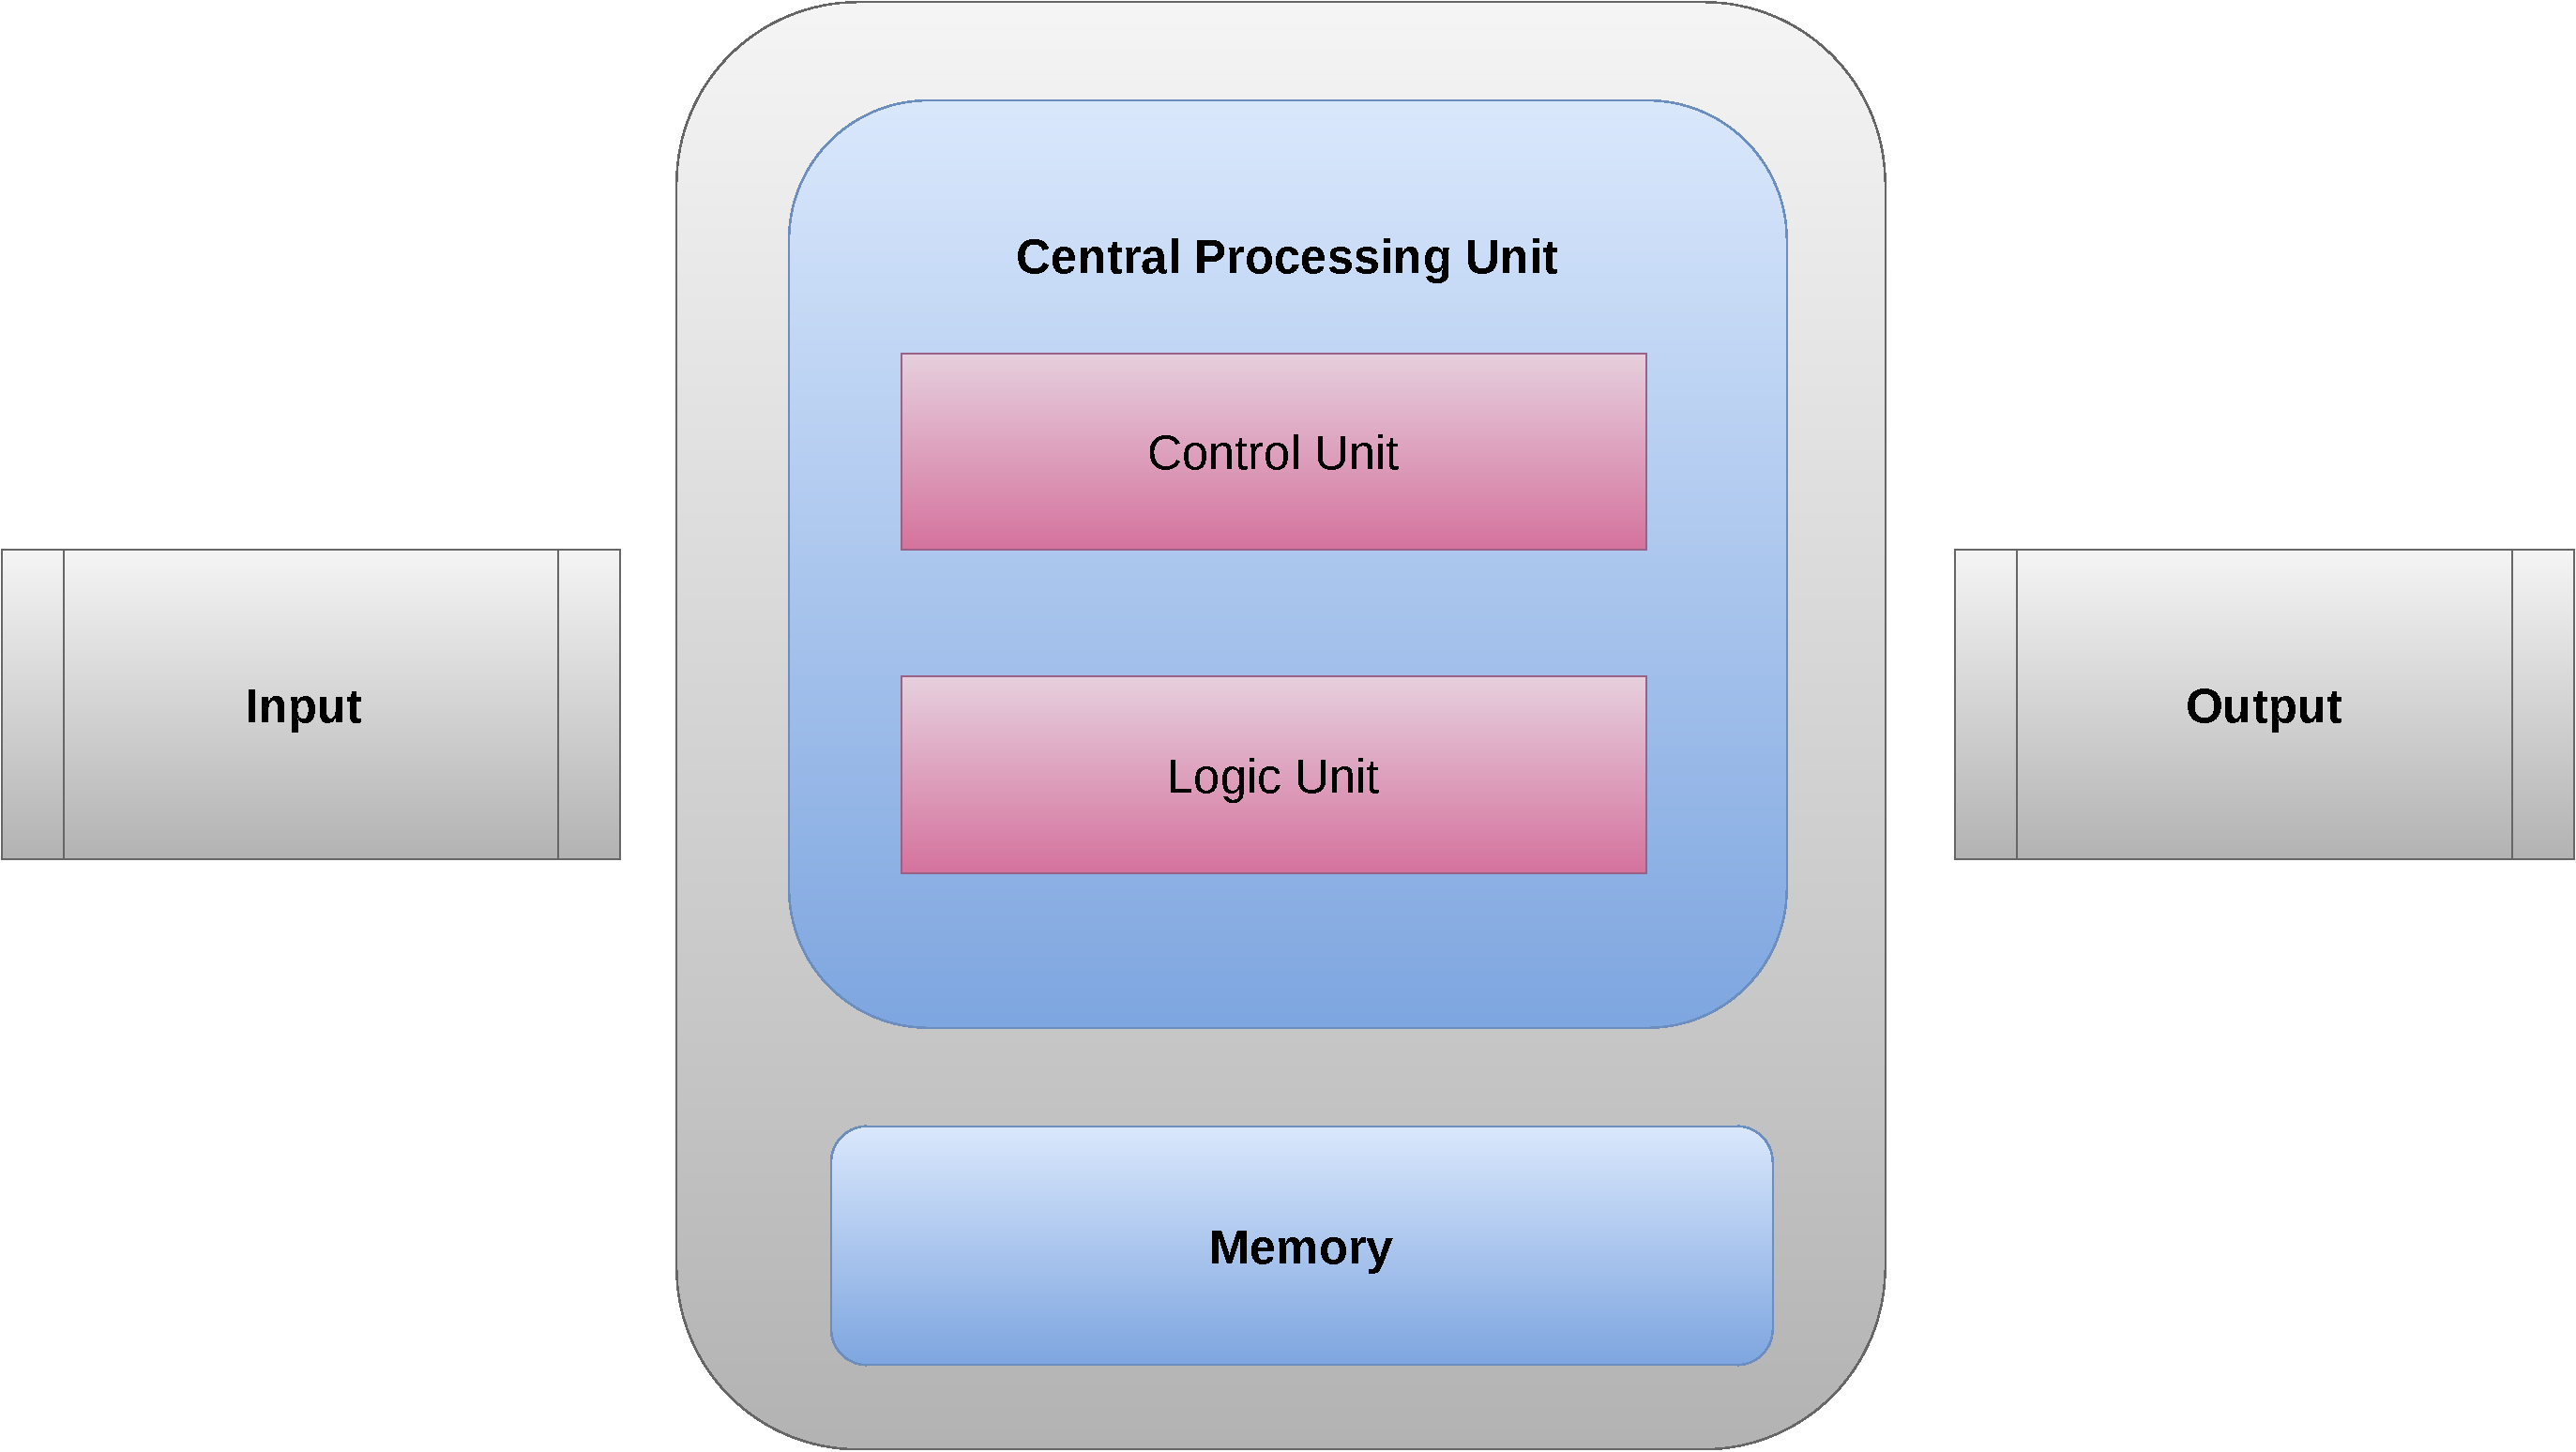
\includegraphics[scale=0.2]{figures/CPU.pdf}
\caption{A schematic representation of a simplified Von Neumann architecture, inspired from paper~\cite{shankar_looking_2017}. The computer is composed of a CPU and a main memory. with an IO mechanism}
\label{figarchivon}
\end{figure}

In 1945, John Von Neumann proposed a digital electronic computer architecture composed of four main components:  a central processing unit, a memory unit, Input/Output (IO) mechanisms and a storage system, as shown in Figure~\ref{figarchivon}. 
Since then, this architectural view has not changed radically. However, the technologies behind the different components have never been the same. 
This minimalist view of a computer has been improved in design and performance, and the number of transistors per chip doubled every 18 months, following Moore's law until the late 2000s. 
Nowadays, instead of putting more electronics into the same chipset, constructors are increasing the computing power per processing unit. The number of cores or processing units (CPUs) keeps increasing, not only in the same nodes but also in distributed configurations, leading us to clusters and supercomputers (see Figure~\ref{figarchisuper}). 
A computing node may contain one CPU socket or more. A CPU is usually a multicore. A node may also contain accelerators such as graphic processing units (GPUs). Several nodes are interconnected with high-speed networks to process large problems. 
For instance, the Frontier supercomputer comprises 8 730 112 cores, spread in nodes of one $3^{rd}$ Gen AMD EPYC CPU and four Purpose-Built AMD Instinct 250X GPUs. CPUs and GPUs are interconnected with AMD Infinity Fabric, and the nodes are interconnected with multiple Slingshot NICs providing 100GB/s network bandwidth\cite{frontier}, Figure~\ref{figfrontierdiag} shows a diagram of a Frontier node. 

\begin{figure}[tb]\centering
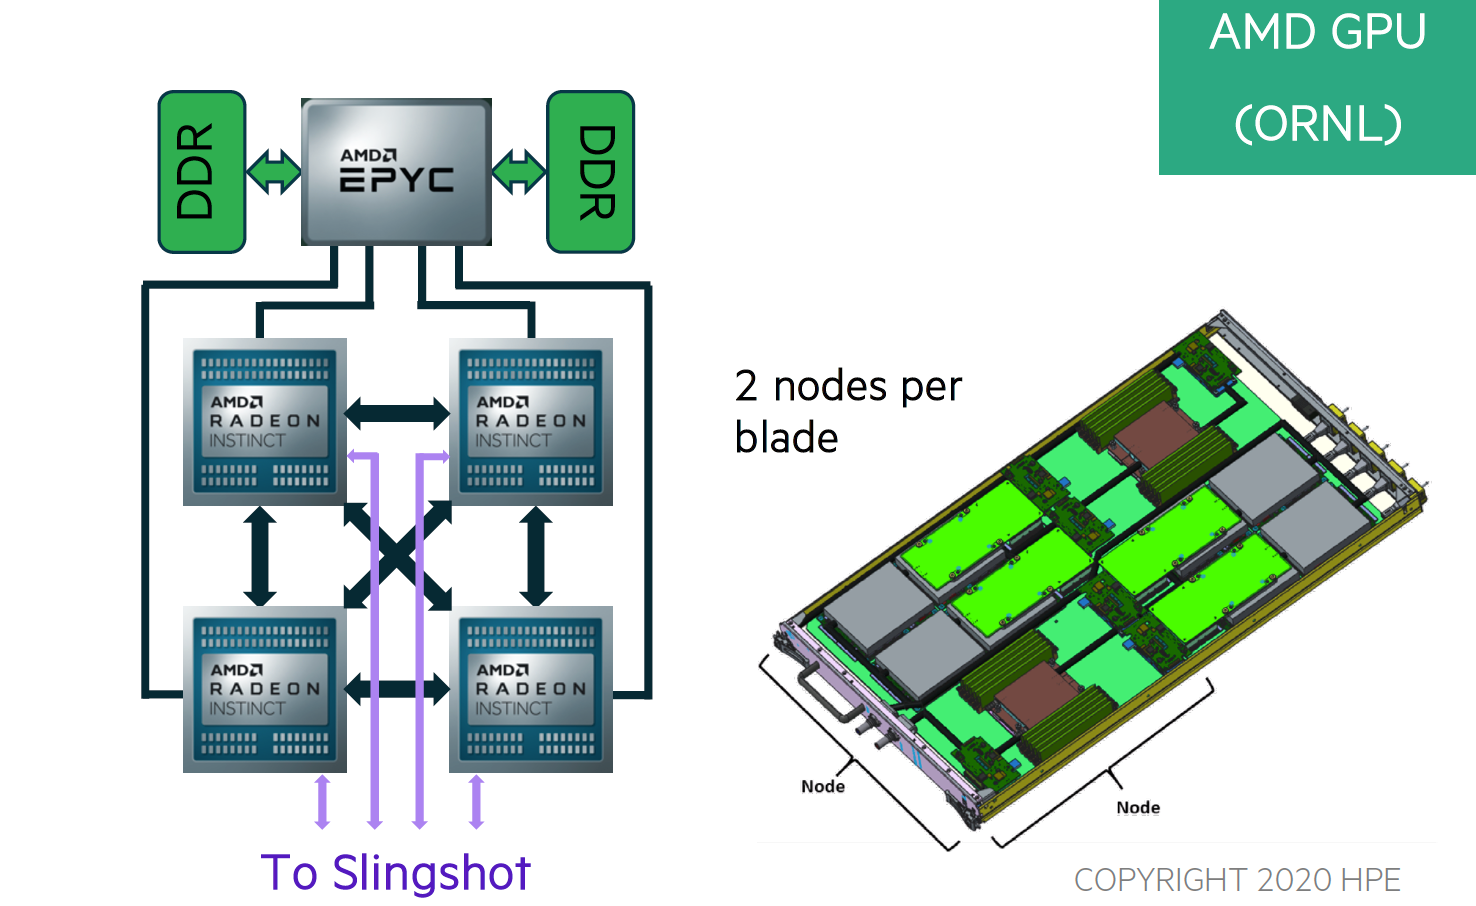
\includegraphics[scale=0.25]{figures/frontier_node_diagram_lr.png}
\caption{Frontier's node diagram, (Figure from~\cite{frontier})}
\label{figfrontierdiag}
\end{figure}

There are many other interconnect systems used in supercomputers. Figure~\ref{figinterconnect} shows the interconnect family system used in the TOP500 supercomputers in November 2022. The most used is Ethernet with 46.6\% usage, followed by Infiniband with a percentage of 38.8\% and Omnipath with 7.2\% and others. In Figure~\ref{figinfiniband}, we show the roadmap of the Infiniband for 1x, 2x, 4x, and 12x port widths with bandwidths reaching 600Gb/s data rate in the middle of 2018 and 1.2Tb/s data rate in 2020.

\begin{figure}[hb]\centering
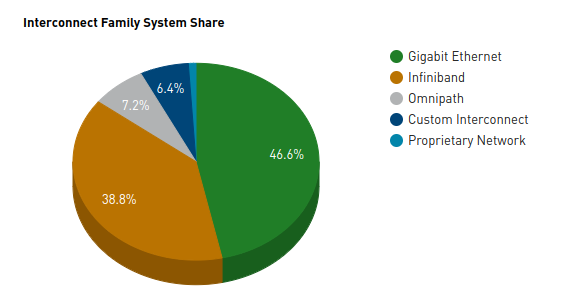
\includegraphics[scale=0.5]{figures/interconnect.png}
\caption{Interconnect family system share in TOP500 2022 list (Figure from Top500~\cite{top500})}
\label{figinterconnect}
\end{figure}


\begin{figure}[tb]\centering
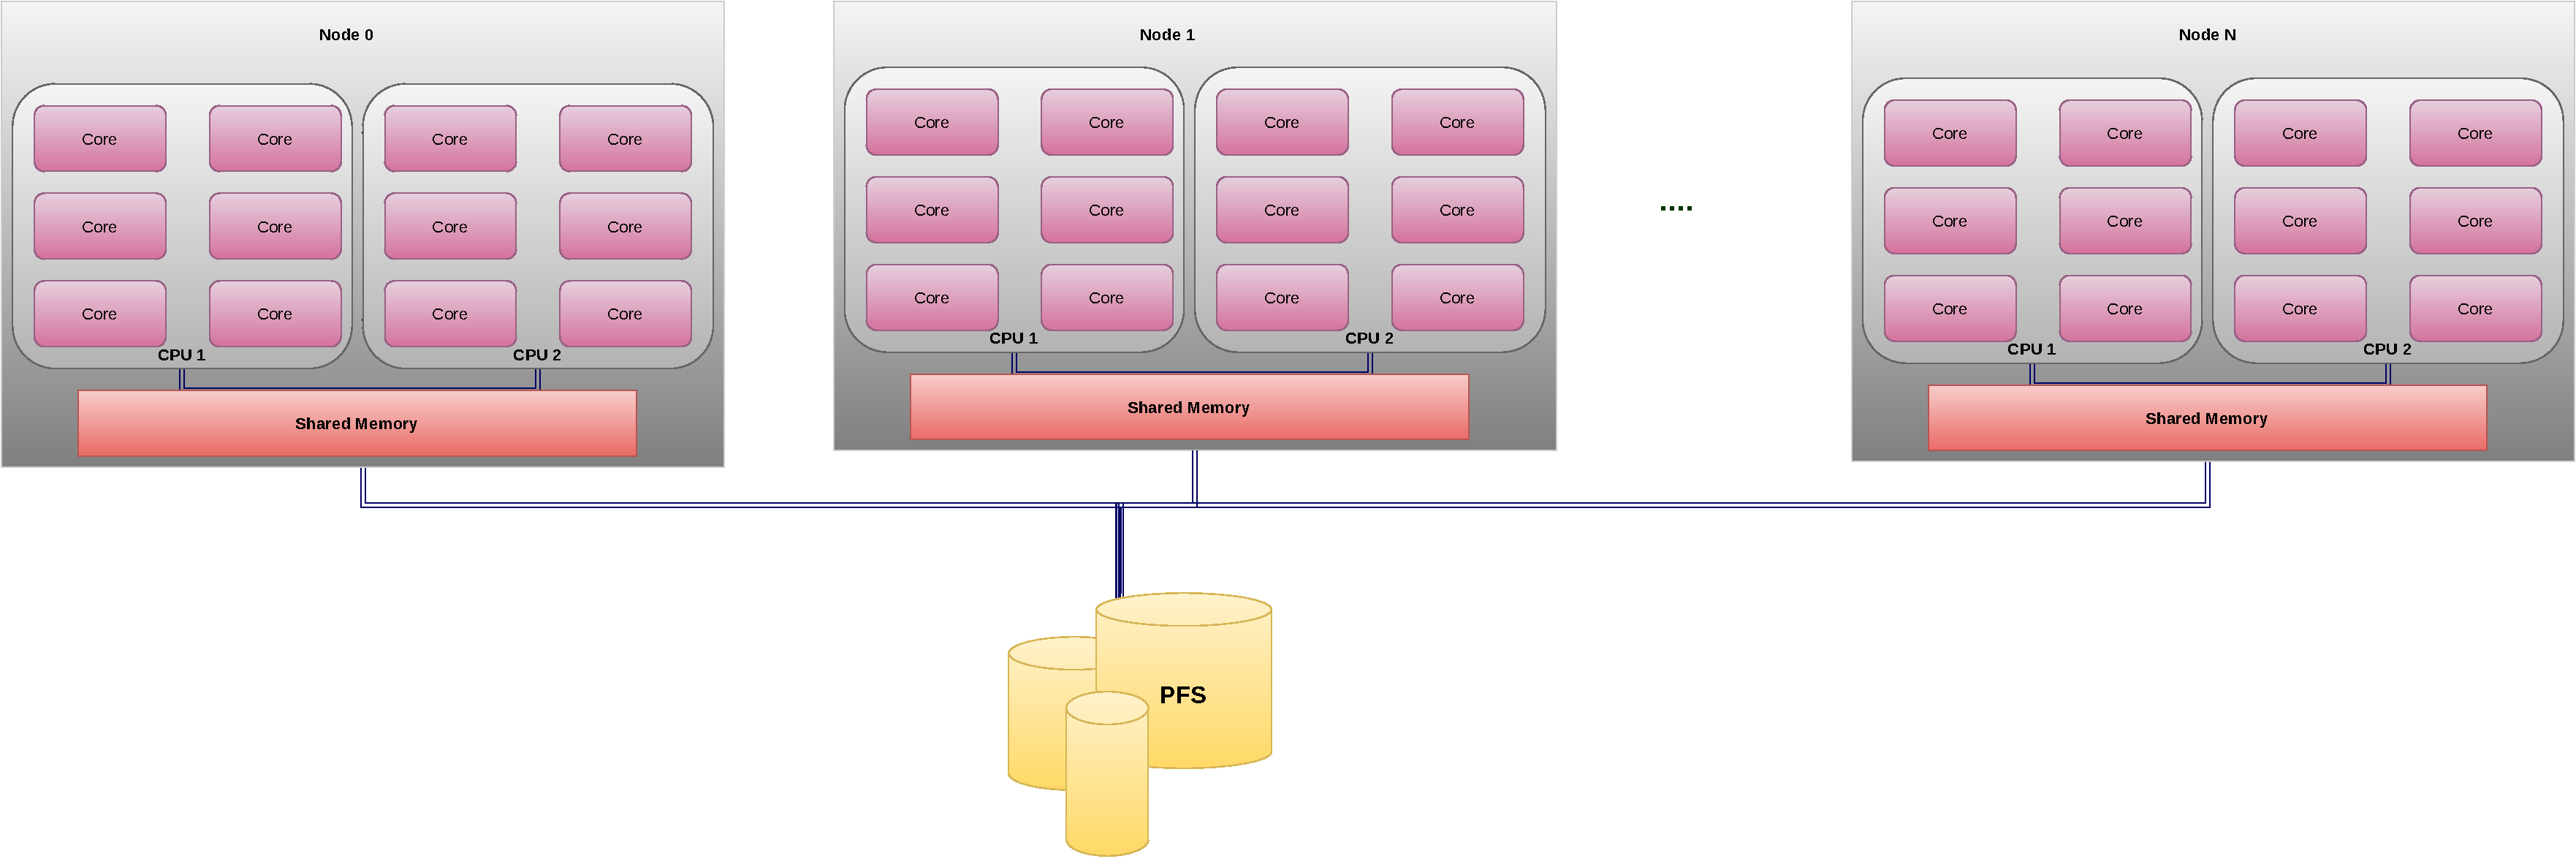
\includegraphics[scale=0.25]{figures/supercomputer.pdf}
\caption{A schematic architecture of a supercomputer represented by compute nodes interconnected. Each node contains two CPUs with six cores. And all the nodes a connected to a parallel file system represented in this picture as shared disks. Figure inspired from~\cite{yan_comparison_2018}}
\label{figarchisuper}
\end{figure}

\begin{figure}[ht]\centering
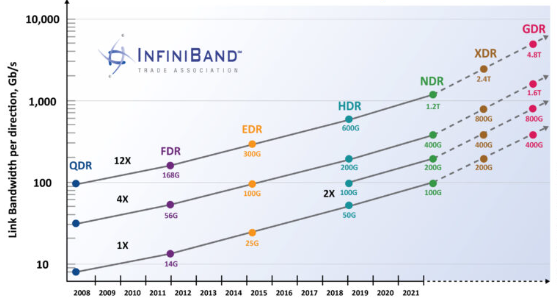
\includegraphics[scale=0.5]{figures/infiniband.png}
\caption{The InfiniBand trends for 1x, 2x, 4x, and 12x port widths with bandwidths reaching 600Gb/s data rate in the middle of 2018 and 1.2Tb/s data rate in 2020, (Figure from~\cite{infiniband}).}
\label{figinfiniband}
\end{figure}

%\hide{
%\begin{figure}[ht]\centering
%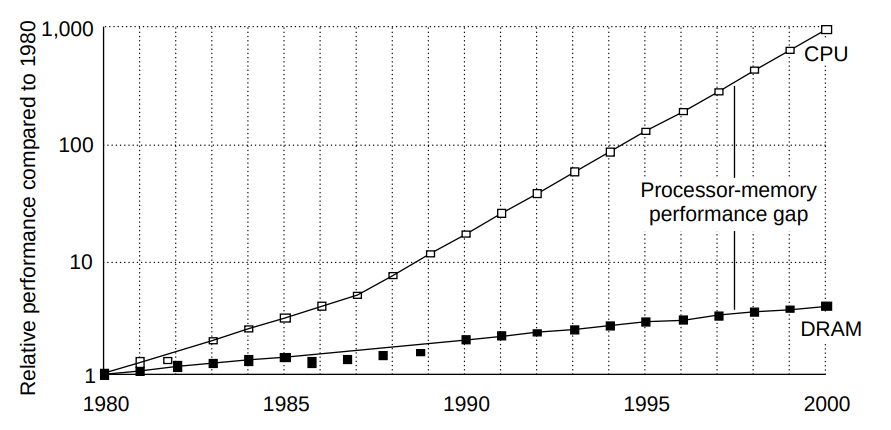
\includegraphics[scale=0.5]{figures/gap.png}
%\caption{The widening gap between CPU performance and memory %bandwidth between the 1980s and 2000~\cite{592312}}
%\label{figgap}
%\end{figure}
%}

\begin{figure}[ht]\centering
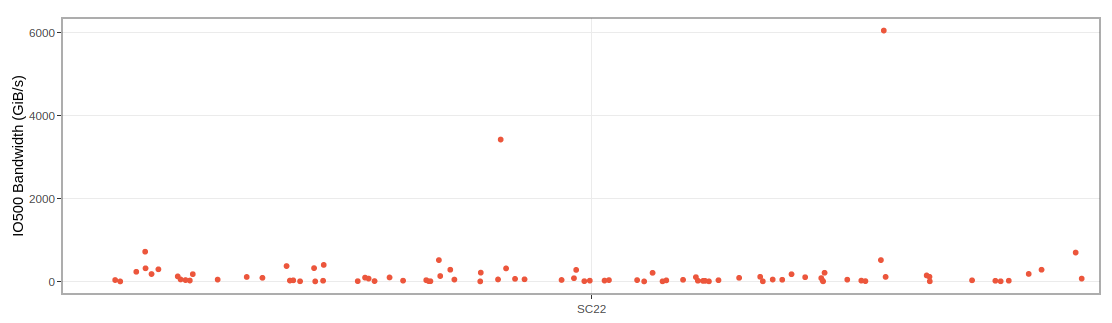
\includegraphics[scale=0.3]{figures/top500.db.png}
\caption{IO500 Bandwidth for November 2022, (Figure from IO500 list~\cite{io500}).}
\label{figioBW}
\end{figure}

The computing power offered by supercomputers generates more precise and huge amounts of data. In addition to an eventual small local storage per node, we find parallel storage servers interconnected together to form a larger storage system. 
A parallel file system (PFS) is software that manages the storage and accesses the data in those distributed servers simultaneously and efficiently. The most used parallel file systems in supercomputers are the open-source Lustre\cite{lustre} file system and IBM  Spectrum Scale or previously named General Parallel File System (GPFS)\cite{gpfs}.   

 While computing power doubles each 12-18 months, storage bandwidth does not.
For a 3Ghz CPU whose average clock cycle is 0.3ns. The latency to access the main memory is between 70-100ns. Random Access Memory (RAM) accesses are two orders of magnitude slower than CPUs, and IO operations are even slower as they take between 1-10ms.
Figure~\ref{figioBW} shows the IO bandwidth for the IO500 supercomputers registered in November 2022. Note that most of the points are situated around 500GiB/s.    
In addition to the huge latency to access a PFS, it is usually shared between several applications running in the supercomputer. If those applications perform IOs simultaneously, then IO performance drops.  


\subsubsection{IO Bottleneck}\label{sec:iobottleneck}

The problem of IO performance comes from three main problems together: the gap between CPU performance and storage bandwidth, the fact that the parallel file system is shared between multiple users and the huge amount of data generated by simulations in some fields.  

One can consider improving the IO performance or reducing the data size to write to reduce the IO bottleneck. We find already in the literature work that dedicates cores or staging nodes for IO operations to reduce the IO jitters on the time-to-solution or send the data to faster memories such as local Solid-State Drives (SSDs) rather than the PFS. 
The second possibility is to reduce the amount of data to write to disk. The easiest way is to make selections on the global domain, such as time sampling, and write only what scientists think is relevant. 
Those decisions are made at the beginning of the simulation usually. Thus a good understanding of the simulated phenomena is necessary but not enough to capture all interesting or rare events. 
The last possibility is to process the data as it is generated and only keep the results. This approach is called in situ processing; it uses the same computing resources as the simulation. 
We have opted for this last possibility: to perform in situ processing to bypass frequent disk accesses and avoid the IO bottleneck for several reasons, such as keeping only small and meaningful data, usually with enough information to keep the study interesting; being able to have online information about how the simulation progress, so activating steering or specific actions if needed; fully leverage the HPC platform and use the resources efficiently.  
Note that in in situ processing, we take advantage of the aggregated interconnect bandwidth of all used nodes instead of being limited to fixed bandwidth (storage bandwidth) as in post hoc processing.

\subsection{High-Performance Data Processing}

\begin{figure}[tb]\centering
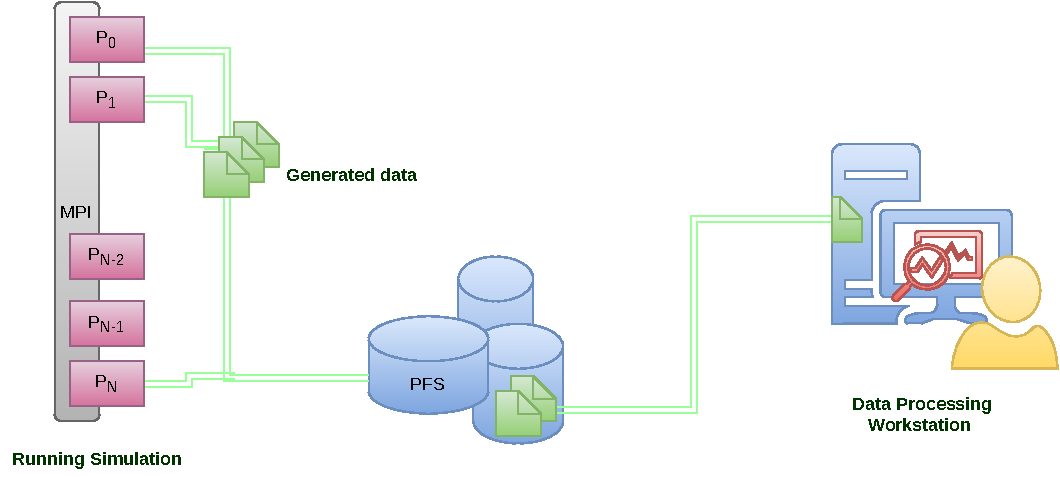
\includegraphics[scale=0.9]{figures/posthoc.pdf}
\caption{schematic view of post hoc processing workflow. In this figure, there are three main entities: the simulation represented by $N+1$ processes, the parallel file system, and a separate desktop computer where analytics are performed.  
The workflow is represented by two main steps: the simulation step, which is concluded by writing the generated data to the parallel file system, and the post-processing step, which starts at the end of the simulation. In this scheme, the generated data is sent to a separate desktop computer where analytics are performed.}
\label{figposthoc}
\end{figure}

HPC numerical simulation is the execution of a program that models a phenomenon in general or the behaviour of an object under specific conditions. The objective is to study and understand aspects of the problem and optimize the underlying industry or contribute with new findings to general science.  The data generated by a scientific application needs to be processed  to understand the phenomenon under study. The classic way to process that data is to save it first to disk and then read it back for post-processing (Section~\ref{sec:posthoc}). 
However, simulations generate dozens of terabytes per hour in some fields, such as weather forecasts and nuclear fusion. Saving all the generated data is impossible both in terms of memory size and time to save to solution because of the IO bottleneck. Moreover, in traditional workflows, the generated data is often processed using sequential Python codes, which is better to replace with parallel codes for larger datasets. However, Python is still one of the best languages and environments for engineering and scientific computing, as it helps to write nontrivial computational programs without getting too bogged down in syntax and compilation time lag~\cite{4160250_python_for_scientific_computing}.
To avoid the IO bottleneck and fully leverage the HPC platform, one can perform in situ processing(Section~\ref{sec:insitu}), which consists in processing the data as close as possible to where and when it is generated. In other words, the data is processed on the same platform where the simulation runs without going through the disk.

\subsubsection{Post Hoc Processing}\label{sec:posthoc}

Post-processing, also known as post hoc or offline processing, refers to analysing or visualizing the generated data at the end of the simulation. The generated data is saved into files in the PFS first, then read back for post-processing in a second step, usually in a separate computing environment. 
In post hoc workflows, the raw data written to disk has to be transformed to extract meaningful physically-based features of interest that will be visualized and analysed in the post-processing step.  

The raw data can be written to one or several files, and one can consider one of those organizations of the data: one file per process over time, one file per process per timestep,  one file per timestep for all the processes, and finally, one file for the whole simulation. Depending on the simulation duration, the number of processes collaborating, and the data size, the choices may be different. For instance, if we deal with a large simulation generating terabytes per timestep, using a single file of the whole simulation may not be the best solution. 

Several IO libraries and file formats are used in HPC, such as MPI-IO~\cite{mpiio}, ADIOS~\cite{lofstead_insights_2013_adios, godoy_adios2_2020}, HDF5~\cite{Folk1999HDF5}, NetCDF~\cite{1592942_netcdf} and so on. However,  HDF5\footnote{https://www.hdfgroup.org/solutions/hdf5/} and NetCDF\footnote{https://www.unidata.ucar.edu/software/netcdf/} are the most common for their performance, flexibility and the possibility to perform parallel IOs. 
  
Figure~\ref{figposthoc} shows a typical post hoc workflow where a running simulation saves the generated data into files in the PFS. Then the files are sent to a data analytics workstation to be processed. 
Scientists may perform either visualization or other any other analysis of the data. Usually, sequential Python codes using already available libraries, such as NumPy~\cite{van2011numpy}, Pandas~\cite{mckinney2010data}, Scikit-learn~\cite{pedregosa2011scikit, kramer2016scikit} and others, are common. 

When the simulations generate large amounts of data, one can take advantage of the existing big data tools to process the data in parallel to reduce the time of the analysis. Nowadays, a large list of frameworks can be found, such as \dask, Ray, Parsl, Spark, Hadoop, PyCOMPSs and so on.   
In this work, we will focus on using the big data framework called \dask distributed for data analytics. However, depending on the needs, any other framework can be considered to process the generated data.
Listing~\ref{numpy}, shows an example of a sequential post hoc code that analyses an HDF5 dataset. It uses the incremental principal components analysis (IPCA) model from the scikit-learn Python library. Listing~\ref{post} shows the equivalent parallel code written using \dask distributed that offers an equivalent parallel implementation of scikit-learn called Dask\_ml. Note that the Listings are almost similar, thus the easiness of porting sequential Python codes to parallel ones with \dask, which is one of the motivations to use \dask in this work.   
More details about \dask are given in Section~\ref{sec:dask.distributed}.

\begin{lstlisting}[float, label=numpy, language=python, caption=Sequential post hoc data analysis with scikit-learn]
from sklearn.decomposition import IncrementalPCA
import json
import h5py
# Load data from HDF5
ds = h5py.File('data.hdf5',mode='r')['dataset']
pca = IncrementalPCA(n_components=2, copy=False, svd_solver='randomized')
# process each time-step independently
for step in range(0, 10):
      pca.partial_fit(ds[step,:,:])
print(pca.explained_variance_)
\end{lstlisting}

\begin{lstlisting}[float, label=post, language=python, caption=Parallel post hoc data analysis with \dask. Lines differing from the analysis of Listing~\ref{numpy} are highlighted]
|\hlline|import dask.array as da
|\hlline|from dask_ml.decomposition import IncrementalPCA
import json
import h5py
|\hlline|# Connect to Dask
|\hlline|sched = json.load(open('sched.json'))
|\hlline|client = dask.distributed.Client(sched["address"])
# Build a lazy array descriptor from HDF5
ds = h5py.File('data.hdf5',mode='r')['dataset']
|\hlline|ds = da.from_array(ds, chunks=(1,4096,4096))
pca = IncrementalPCA(n_components=2, copy=False, svd_solver='randomized')
for step in range(0, 10):
      pca.partial_fit(ds[step,:,:])
print(pca.explained_variance_)
\end{lstlisting}


To summarize, post hoc workflows are easy to set up. They keep decoupled the simulations and the data analytics by passing the data via files. Moreover, one can take advantage of the available ecosystems to process the data, especially using the Python libraries such as NumPy, Pandas, Scikit-learn and others, or pythonic parallel frameworks such \dask, Ray and so on when dealing with big data. However, today the IO bottleneck stands as a barrier between HPC and data analytics going through the disk (post hoc processing). In the following section, we present another data processing workflow scheme called In situ, characterized by its performance compared to post hoc workflows as it avoids unnecessary data communications and IOs.      



\subsubsection{In situ Processing}\label{sec:insitu}

The in situ\cite{InSituLiuMa:2007, in_situ_methodes} paradigm stands for processing the data generated by a simulation code as close as possible to when and where it is generated. In other words, data analytics are performed simultaneously in the same computing platform as the simulation.
In situ workflows allow sharing of data between the simulation and the analytics. Thus, they reduce unnecessary data communications and IOs. Moreover, they allow data reduction and feature extraction to minimize the data memory size to save.   

\begin{figure}[tb]\centering
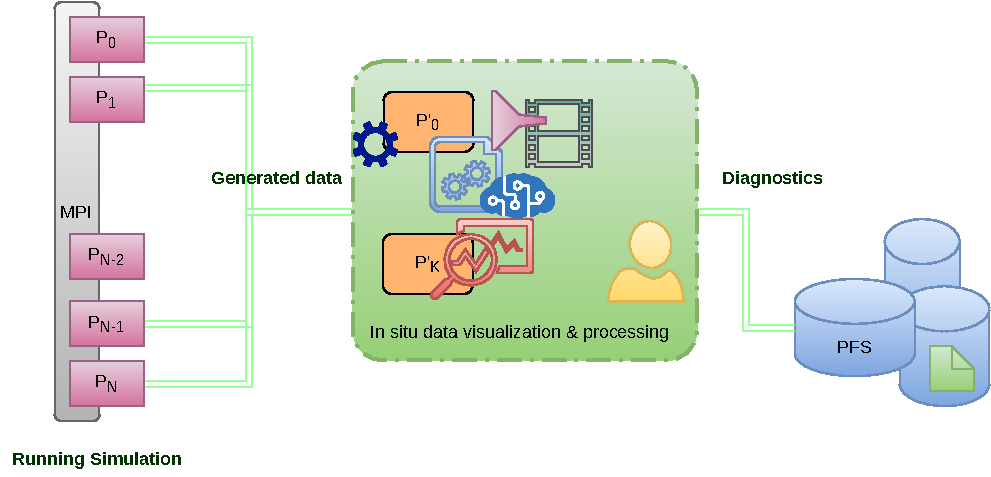
\includegraphics[scale=0.9]{figures/insitu.pdf}
\caption{A schematic view of an in situ processing workflow. The simulation is represented by a set of MPI processes. They generate data which is sent to staging resources to perform analytics that generates diagnostics and reports that are written to the parallel file system. Note that in situ workflows happen in the same computing platform as the simulation but not necessarily in distinct nodes.}
\label{figinsitu}
\end{figure}

Figure~\ref{figinsitu} shows a typical in situ workflow, where the running simulation feeds the in situ analytics programs with the data it generates. Those analytics programs range from simple local Python code to IA inference or 3D rendering and visualization. By the end of the analytics, only interesting results and diagnostics are saved to disk. 

The simplest way to perform in situ analytics is o embed the analytics routines into the simulation code. However, this approach reduces the separation of concerns and may quickly produce an unmaintainable code. A cleaner way to do that is to decouple the analytics from the simulation. One can use data-handling libraries to access the simulation data and share it with external codes for analytics.   
 
There are several other ways to perform in situ analysis, either by time (Section~\ref{sec:timesharing}) or space (Section~\ref{sec:spacesharing}) sharing with the simulation processes. 
Analytics can share the same thread or process or just the same node with simulation; the processing in those cases is called in situ. If they only share the same supercomputer, and the data is sent to staging nodes, then we say in transit processing. It is also possible to perform both in situ and in transit processing in the same workflow.

In situ analytics allow data reduction and feature extraction while the simulation is running, which makes it easy to steer the simulation and trigger further analysis if needed. For instance, if a rare event is detected in situ, the simulation can be restarted from the last checkpoint, and further analytics may be done to understand further the event formation. This use case may be possible in post hoc workflows only if all the data is kept on the disk, which is not always the case. 
Moreover, instead of automatically reducing the size of raw data, such as having an output for each $N$ timestep, which may lead to missing interesting events, in situ workflows allow a smarter selection of output data. Consequently, in situ does reduce not only the size of the data but also allows a smarter selection of interesting ones.



\paragraph{Time Sharing}\label{sec:timesharing}

In time-sharing scenarios, the same cores are used by both simulation and the in situ analytics processes. Synchronous and asynchronous executions may be performed. 

\begin{itemize}
    \item \textbf{Synchronous Execution}
    In synchronous scenarios, the simulation is stopped periodically to perform analytics tasks. In a typical cycle, the cores are used for the simulation first, and when the data is ready for analytics, those cores are used for analytics. These two steps are repeated until the end of the simulation (Figure~\ref{figinsitusynch}).
    
    \begin{figure}[tb]\centering
    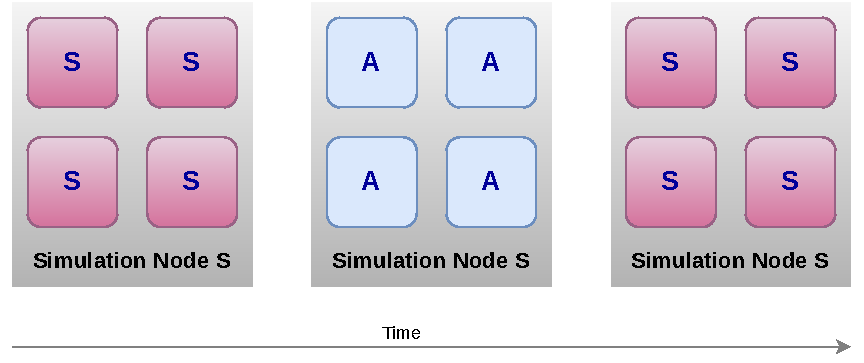
\includegraphics[scale=0.9]{figures/insitu_synchronous.pdf}
    \caption{A schematic representation of synchronous in situ execution in a node with four cores. The simulation runs on the cores until an analytics step is reached. The simulation stops, and then analytics takes over. This cycle is repeated until the end of the workflow, (Figure inspired by~\cite{Estelle_integration_2018}).}
    \label{figinsitusynch}
    \end{figure}


    \item \textbf{Asynchronous Execution}
    In the asynchronous scenarios, the cores are over-subscribed for both simulations and in situ analytics. The operating system (OS) scheduler is in charge of co-scheduling the two processes (Figure~\ref{figinsituasynch}). This approach is less efficient because of the contentions on shared resources (such as memory buses and caches..)~\cite{zheng2013goldrush, Estelle_integration_2018}. 

    \begin{figure}[tb]\centering
    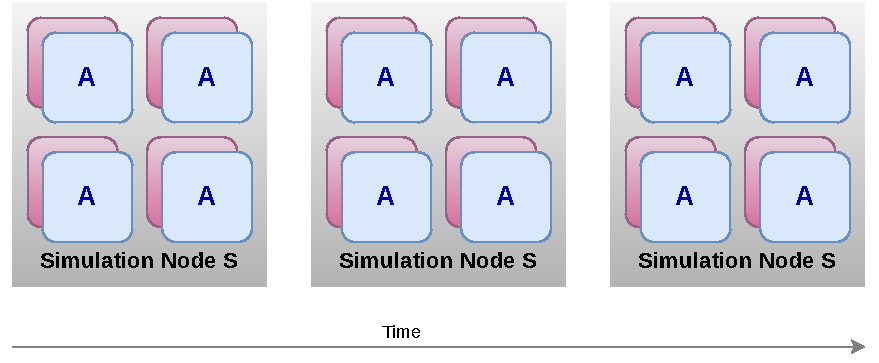
\includegraphics[scale=0.9]{figures/insitu_asynch.pdf}
    \caption{A schematic representation of an asynchronous in situ execution in a node with four cores. The simulation and the analytics are scheduled in the same over-subscribed cores, (Figure inspired by~\cite{Estelle_integration_2018}).}
    \label{figinsituasynch}
    \end{figure}

    In the rest of this section, we will focus only on synchronous scenarios.
    
\end{itemize}

In synchronous scenarios, analytics routines may be directly embedded in the simulation code. In this case, we say that the analytics and the simulation are tightly coupled. This approach is not recommended, as analytics routines will likely changing very quickly, unlike the simulation. If the code is not well designed, such an approach may produce an unmaintainable code.
To avoid such a situation, one may consider the separation of concerns design principle to provide a loosely coupled solution: each part of the workflow only computes what is designed for and provides an interface to communicate with other sections.

We have mentioned the separation of concerns here because it is one of the most important design principles and one of the objectives of this work.

\paragraph{Space Sharing}\label{sec:spacesharing}
In space-sharing scenarios, the resources are shared between simulation and analytics tasks. The analytics uses distinct cores (see Figure~\ref{figinsituhelper}), which are usually called helper cores. The simulation always runs on fewer cores, but still, it uses more than the analytics. However, the performance loss is generally less than the ratio of confiscated cores \cite{zheng2013goldrush, dorier_damaris_2012, Estelle_integration_2018}.

Because distinct resources are used, the analytics are usually \textbf{asynchronous}, and the data to be analysed is copied/transferred  at least once before the simulation resumes for the next step. The analytics cores used for analytics may be located on the same node as the simulation or in distinct nodes. In this last case, the analytics are called \textbf{in transit} analytics ( Figure~\ref{figintransit}). 
\begin{figure}[tb]\centering
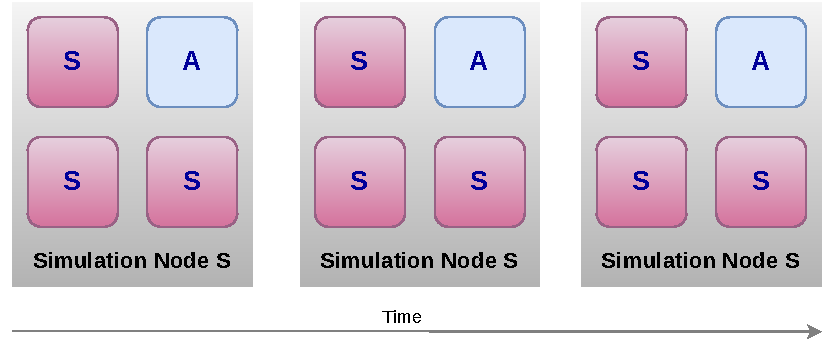
\includegraphics[scale=0.9]{figures/insitu_helpercore.pdf}
\caption{A schematic representation of asynchronous in situ execution in a node with four cores: the simulation runs on three cores, and the analytics on one helper core. The simulation and the analytics are collocated in the same node, (Figure inspired by~\cite{Estelle_integration_2018}).}
\label{figinsituhelper}
\end{figure}

\begin{figure}[tb]\centering
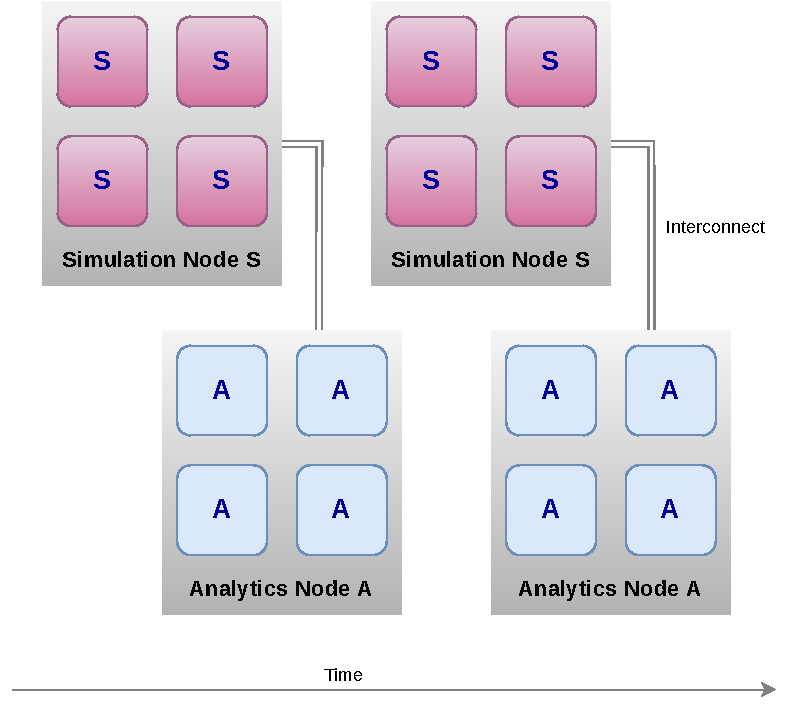
\includegraphics[scale=0.8]{figures/intransit.pdf}
\caption{A schematic representation of in transit workflow. The simulation and the analytics run on distinct nodes. When a simulation step is completed, and data is ready to be processed, it is sent to analytics nodes over the network. Note that the simulation and the analytics node are located in the same computing platform, (Figure inspired by~\cite{Estelle_integration_2018}).}
\label{figintransit}
\end{figure}

\subsubsection{Heterogeneous Workflows}
Because all configurations have their pros and cons, heterogeneous architectures are possible: either in terms of analytics placement or workflow synchronicity. One can perform synchronous in situ analytics, where the analysis routines are embedded in the simulation code, followed by in transit analytics on a staging area. This example is interesting, for instance, when the in situ routines reduce the size of data that needs to be sent to the staging nodes, and the in transit routines are heavy slow analytics algorithms.  

\subsubsection{Discussion}
In situ processing is a good alternative to traditional post hoc workflows. They optimize several aspects of the HPC workflows, namely: the IOs, data communication and processing, the size of the output, and the workflow duration, thus, energy consumption.
%The most critical issue that would block scientific discovery through HPC is the IO bottleneck. 
In situ workflows avoid the IO bottleneck by avoiding unnecessary IOs. They bypass disk accesses and avoid unnecessary data communications by sharing the same computing platform as the simulation. 
In addition, they allow data reduction and feature extraction while the simulation is running, which makes it easy to steer the simulation and trigger further analysis if needed. Moreover, instead of automatically reducing the size of raw data, such as having an output for each $N$ timestep, which may lead to missing interesting events, in situ workflows allow a smarter selection of output data. Consequently, in situ does reduce not only the size of the data but also allows a smarter selection of interesting ones.

As we have presented in the previous sections, in situ analytics can be performed synchronously or asynchronously with simulation, in the same cores/nodes or in different ones. Each variant has its pros and cons. For instance, synchronous in situ workflows may penalize the simulation if the analytics are relatively long and oversubscribing the core is not better because the OS scheduler may be inefficient on that. Dedicating cores or nodes is better from this point of view because of using distinct resources. However, data flow has to be managed carefully in those cases. 

This work is devoted to working on another important aspect of in situ analytics, which is their setup complexity compared to post hoc workflows. 
This complexity usually derives from the programming model used in in situ tools, which is often the inherited message passing (MPI) model from the host simulation. 

\subsection{Parallel Programming Models}\label{sec:programmingmodel}

In this section, we present two parallel programming models: MPI, which is the most used to parallelize HPC simulations, and a higher-level programming model called distributed task-based paradigm, which is adapted for analytics. We finish with a discussion of how such  higher-programming model could help to reduce the complexity of setting up in situ workflows.

A programming model is a set of concepts and program abstractions associated with a programming interface that is used for modelling and implementing algorithms. It is related to a programming paradigm that represents the theoretical concepts of the model, which may be built on hardware architecture or algorithmic specifications. 
Parallel programming models fit tasks from the parallel application to parallel hardware. They range from the application layer to programming languages, compilers, libraries, network communication, and IO systems\cite{VITOROVIC2014203_parallel_programming_models}.

Increasing the CPU frequency makes applications faster without changing the programming model; it consists in reducing the clock cycle, thus executing more instructions in the same duration. Putting more cores in CPUs, more CPUs in nodes, and pushing the limits to distributed configuration, with or without accelerators introduce changes in the programming model and require new ones. 

There are several attempts to classify programming models~\cite{belikov2013survey, nestmann_building_2017, ketata_parallel_2016, thoman_taxonomy_2018, kasim_survey_2008}, focusing on several criteria such as the architecture (shared or distributed memory), type of parallelism, on abstraction level or productivity.  
The most relevant taxonomy to this work appears in~\cite{belikov2013survey}. It develops a classification over several axes and shows a distribution of parallel programming models across two important dimensions, namely: computation (i.e. the algorithmic solution) and coordination (the management of parallelism), whether they are explicit or implicit, as represented in Figure~\ref{figmodels}. 

\begin{figure}[tb]\centering
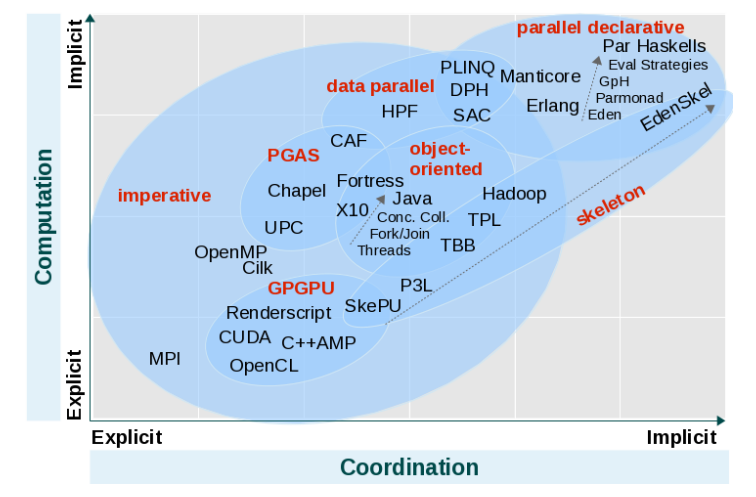
\includegraphics[scale=0.5]{figures/programming_models.png}
\caption{Programming model distribution according to their computation and coordination abstraction level: whether explicit or implicit, (Figure from~\cite{belikov2013survey}).}
\label{figmodels}
\end{figure}

We are interested in two main programming models in this work: the MPI programming model that can implement the Bulk-synchronous parallel (BSP) paradigm, which is one of the most popular parallel programming models for distributed memory systems \cite{BRINSKIY2015305_MPI_3} (Section~\ref{BSP}), and the distributed task-based programming model that is gaining more popularity for its simplicity and productivity as it intends to provide more and more implicit computations and coordination (Section~\ref{sec:taskbased}).


\subsubsection{Bulk Synchronous Parallel Paradigm}\label{BSP}
In \cite{valiant1990bsp}, \textit{Leslie G. Valiant} introduced the bulk-synchronous parallel paradigm as a bridging model between software and hardware for parallel computing. He argued that such a model is analogous to the \textit{Von Neumann} model and would get the same success as this last.
A Bulk-Synchronous Parallel computer combines three attributes : 
\begin{itemize}
    \item a number of \textbf{components}, each performing processing and/or memory functions,
    \item a \textbf{router} that delivers messages point to point between pairs of components,
    \item facilities for \textbf{synchronizing} all or a subset of the components at regular intervals of $L$ time units where $L$ is the Periodicity parameter.
\end{itemize}

A BSP machine can be implemented using the well-known communication interface: Massage Passing Interface (MPI), where the components are defined as a set of $P$ processes that share a common communicator. Each process has its separate local memory, performs a set of computations on its local data, and then exchanges some results with other processes. A local/global synchronization is performed periodically. Figure \ref{figmpi} shows an execution flow over time of an MPI program. 

The MPI programming model suits very well the scientific applications where models are regular. The global domain is decomposed statically and explicitly within the processes. Each process has its local buffers updated as the simulation progresses, and parts of those buffers are exchanged with a subset of processes when needed. In this work, we focus on the MPI implementation of the BSP paradigm.

\begin{figure}[tb]\centering
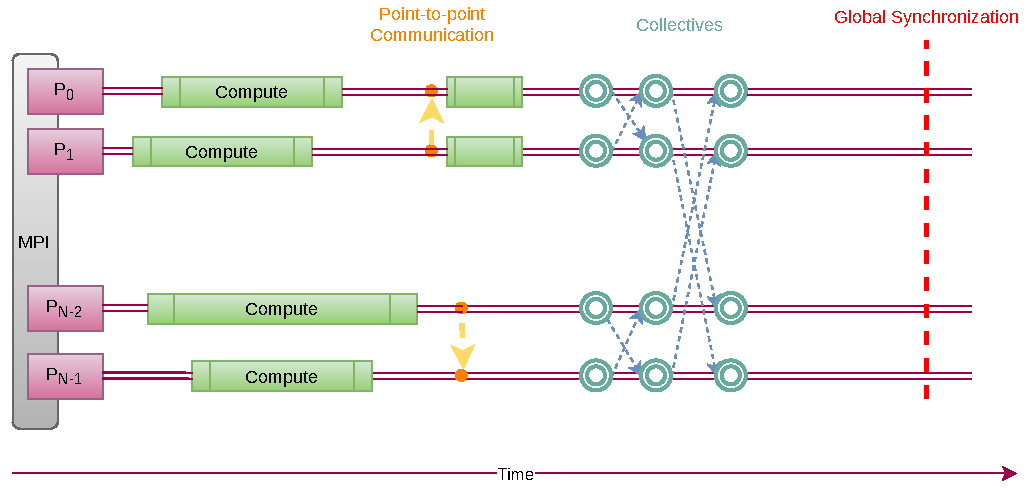
\includegraphics[scale=0.9]{figures/MPI.pdf}
\caption{Execution flow of an MPI program represented by $N$ processes. Compute, communication and synchronization regions have been represented over time, inspired by~\cite{mpi_report}}
\label{figmpi}
\end{figure}

Unlike several programming models that introduce new complex concepts, MPI was built using a relatively small number of well-defined and forward-looking concepts\cite{traff_recent_2012}. In the MPI-1 standard, an MPI process runs a program in its private address space and can communicate either through point-to-point message passing with another process or through collectives. 
The MPI standard has been then extended in several ways; however, using MPI may only require knowing a few concepts. 
In addition to the strong base of MPI, it was designed to work with other tools. This characteristic is vital because the complexity of software and hardware keeps increasing. It also supports component-oriented software, thanks to communicators and groups, which is very important in designing modular or hierarchical code. Moreover, MPI is a complete model that can be used to write any parallel algorithm and is portable and can be used on platforms ranging from laptops to supercomputers\cite{goos_learning_2001}. All those characteristics make MPI perfectly fit high-performance applications and be a widely used model in HPC.

Note that in MPI, the resource allocation and scheduling of the computations to processes are managed explicitly; while this is not a big issue for regular algorithms, it can quickly become complicated to manage for irregular ones.


\subsubsection{Distributed Task-based Programming}\label{sec:taskbased}

Despite MPI success and efficiency, it is not the most suited model to parallelize irregular algorithms. This category of problems is characterized by irregular data structures and control patterns. Using static decomposition to parallelize them is not trivial. Higher-level programming models, such as task-based programming, reduce this complexity by cutting the computation into a set of tasks, and then a runtime dynamically schedules them. 

Task-based paradigm has been introduced first in the shared memory context, Cilk~\cite{cilk5}, OpenMP~\cite{openMP} and Intel TBB~\cite{Robison2011tbb} are examples of shared memory task-based tools. Task-based programming was then extended to distributed memory in~\cite{kooburat_extending_nodate}, and used to design several frameworks and tools; we will give more examples in Section~\ref{sec:task-based-frameworks}. 


In the task-based paradigm, we define three main concepts:
\begin{itemize}
    \item A number of \textbf{stateless tasks}: a task is defined as a sequence of instructions within a program that can be processed concurrently with other tasks in the same program\cite{thoman_taxonomy_2018}. A task has inputs and outputs. It can be either fine-grained or of a coarser granularity. 
    
    \item \textbf{Dependencies} between tasks. A task can only be executed when all its dependencies are resolved,
    
    \item An \textbf{engine} that manages and schedules the execution of those tasks on a set of physical processes, which is usually called a scheduler,

    \item \textbf{Actor} is another concept that has emerged in several task-based systems. It is a stateful entity. It has internal attributes that may change when receiving messages from the environment. It may react by changing its internal state or/and sending responses. 
\end{itemize}

In the task-based model, an application is split into tasks that are related to each other with dependencies to form a Directed Acyclic Graph (DAG): where the nodes are the tasks, and the edges represent the dependencies (Figure~\ref{figdag}). A task with no input edges is called an entry task, while a task with no output edges is called an exit task\cite{ruadulescu1999complexity}.  
The runtime scheduler analyses the DAG and decides which of the ready tasks to run on the available resources.

\begin{figure}[tb]\centering
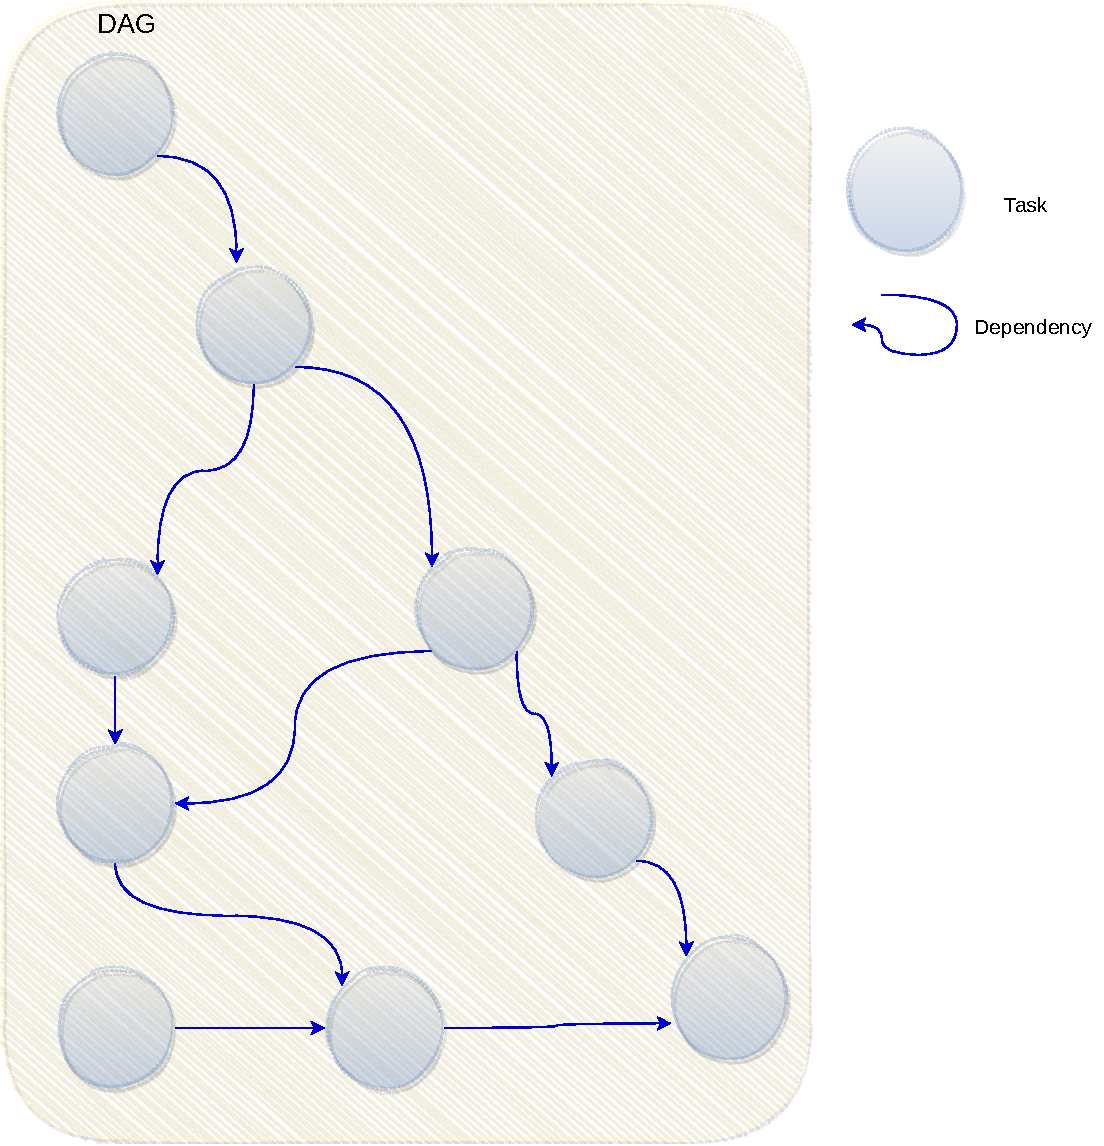
\includegraphics[scale=0.5]{figures/dag.pdf}
\caption{A directed acyclic graph: the nodes represent tasks, and the edges are the dependencies}
\label{figdag}
\end{figure}

One of the main motivations for introducing higher-level models, such as distributed task-based paradigm, is to create higher-level abstractions that make the design and implementation of parallel algorithms easier. The resource and the task scheduling (coordination) are managed by the runtime scheduler implicitly from the user's point of view. 
The task-based models can be less efficient in terms of performance compared to BSP-based models due to the overheads that may be introduced during runtime (due to the dynamic scheduling of tasks and message management at runtime). However, they widely increase productivity with the simplicity they introduce in designing and maintaining non-trivial applications.   

In this work, we have chosen the \dask distributed framework as a distributed task-based tool to study and use, and we present in detail its architecture, task and data management and internal scheduling in Section~\ref{sec:dask.distributed} 


\subsection{Discussion}\label{sec:discussion:programmingmodels}

While in situ processing is a relevant solution to avoid the IO bottleneck, it has several drawbacks, such as the setup complexity of in situ workflows and a priori knowledge needed to write relevant in situ analytics. In this work, we  have a look at the complexity behind in situ workflows.  

Most HPC simulations are written on MPI programming model alongside other models, known as MPI+X, for their efficiency. Thus, most of the existing in situ tools are built on the MPI programming model, which is inherited from the host simulation. However, while MPI+X is the most suited model for the HPC simulations, it does not suit well data processing algorithms for several reasons.
First of all, HPC applications are usually characterized by a regular structure, where the program is a loop where processes usually run the same code and exchange data when necessary with neighbours, update the distributed data structure and synchronize globally. Adopting static and explicit parallelism using models such as MPI is relatively easy to apply and very efficient in terms of performance for such regular programs. 
On the other hand, data analytics algorithms are usually irregular; they may be characterized by one or more of the three types of irregularities, namely: data structures, control structures and communication patterns irregularity\cite{4919639}. When the algorithm manipulates an irregular data structure, such as unbalanced trees, a need for dynamic scheduling and load balancing arises. When the algorithm presents irregular control patterns, synchronous models are not the most efficient. And when the algorithm shows irregular communication patterns, which is usually a result of the two precedent irregularities, non-determinism appears, and static models are not the most suited for such problems. 
Moreover, HPC simulations are programs that model a phenomenon, and the physics or logic behind it is less likely to change over time. It may be subject to improvement but rarely to core changes. Thus spending time/money on improving performance thanks to complex programming models is relevant because such codes are used for a couple of dozen of years.   
On the other hand, data analytics algorithms may change from one study to another and are likely to change more frequently than the simulations themselves; moreover, they are less costly in computation. One would rather choose a less complex or easier model for such programs, even if the model is less efficient. In this work, we have opted for the distributed task-based framework that is both dynamic and asynchronous, with implicit parallelism usually ensured at runtime by a scheduler.   

 All in one, data analytics algorithms are different from simulations in their structure and execution; it is better to adopt a more suited model rather than taking the default option inherited from the host simulation.     

%The user needs to put more effort into programming the new architectures by trying to explore the maximum of parallelism, usually using different programming models. In addition to the constant quest for performance, using these models, the user will need to couple them to perform more complex tasks. 
%Paradigms that are built on different concepts are complicated to couple; one needs a deep understanding of the concepts and the implementations to do this task.  
%In this work, we propose a bridging model between BSP and distributed task-based paradigm to simplify in situ processing.  

%%%%%%%%%%%%%%%%%%%%%% 02/03/2023%%%%%%%%%%%%%%%%%%%%%%%%%
\section{In Situ Analytics}
In this section,
we present in the following sections some well-known in situ tools and frameworks, how the task-based paradigm has been used in the in situ workflows and finally, have a look at the big data frameworks already used for in situ analytics. We will have a discussion after each section to compare the presented tools.

\subsection{General In Situ Frameworks}\label{sec:insitu:tools}
%ADIOS I, II, Damaris, FlowVR, decaf, bredala, filtring, smartsim, 

The in situ paradigm, as already presented, appeared for the first time in the paper of Kwan-Liu Ma \textit{et al.} and has been applied first to scientific visualisation~\cite{InSituLiuMa:2007}. In this paper, which appeared in 2007, the authors already observed and declared that with the growing power of supercomputers and to be able to maximize the utilization of the data generated by simulations, one has to minimize or avoid IOs that are becoming a performance bottleneck. 
Thanks to this work,  most scientific visualization frameworks that are meant for high-performance computing support in situ visualization. Paraview~\cite{ahrens_paraview_2005} and VisIt~\cite{childs_visit_nodate, noauthor_about_visit, whitlock2010getting}, which are built on the visualization toolkit VTK\cite{noauthor_vtk, schroeder_visualizing_2000_vtk}, both support in situ visualization thanks to the Catalyst~\cite{catalyst11, noauthor_what_catalyst} and  Libsim~\cite{libsim11} extensions, respectively.

ParaView is an open-source post-processing visualization tool built on MPI. It can run on computing platforms ranging from laptops to Exascale machines and process small to large datasets. Catalyst is an in situ library that enables easy integration of analysis routines within simulation codes.
ParaView Catalyst~\cite{bauer_paraview_2016, noauthor_using_paraview, noauthor_paraview_nodate, cscsch_situ_2022, ayachit2021catalyst} is the name given for catalyst implementation that uses ParaView for in situ analytics. It allows in situ processing and visualization workloads to run synchronously with the simulation by sharing the same data. This data needs to be transformed into VTK data structures by implementing an \textit{Adaptor} to be understandable by ParaView. 
For most simulation codes, the coupling between the main simulation code and the adaptor will only
involve three function calls. The first call initializes Catalyst and the pipelines; the second call performs any
requested co-processing; and the third call finalizes Catalyst
~\cite{catalyst, paraview_catalyst_examples_2022}.

VisIt is another well know visualization tool. It has a plugin architecture that allows to perform a wide variety of data processing operations and also import data from several data formats. It provides an interface for in situ analytics through libsim~\cite{childs_situ_libsim_2022}. Libsim ensures two main functions: it creates an interface  to map simulation data to VisIt format and manage VisIt events~\cite{ dreher_methodes_2015}.
An \textit{Adaptor} is implemented here also if the simulation is not compatible with the VTK data structures used by VisIt. 
Similarly to ParaView, Visit is built on MPI. It has a client/server architecture where one or more clients connect to a viewer, and remote servers run the in situ routines on the HPC plateform~\cite{noauthor_visit_works}. Figure~\ref{figvisit} shows VisIt architecture where the input data is either the PFS or a running simulation.

\begin{figure}[tb]\centering
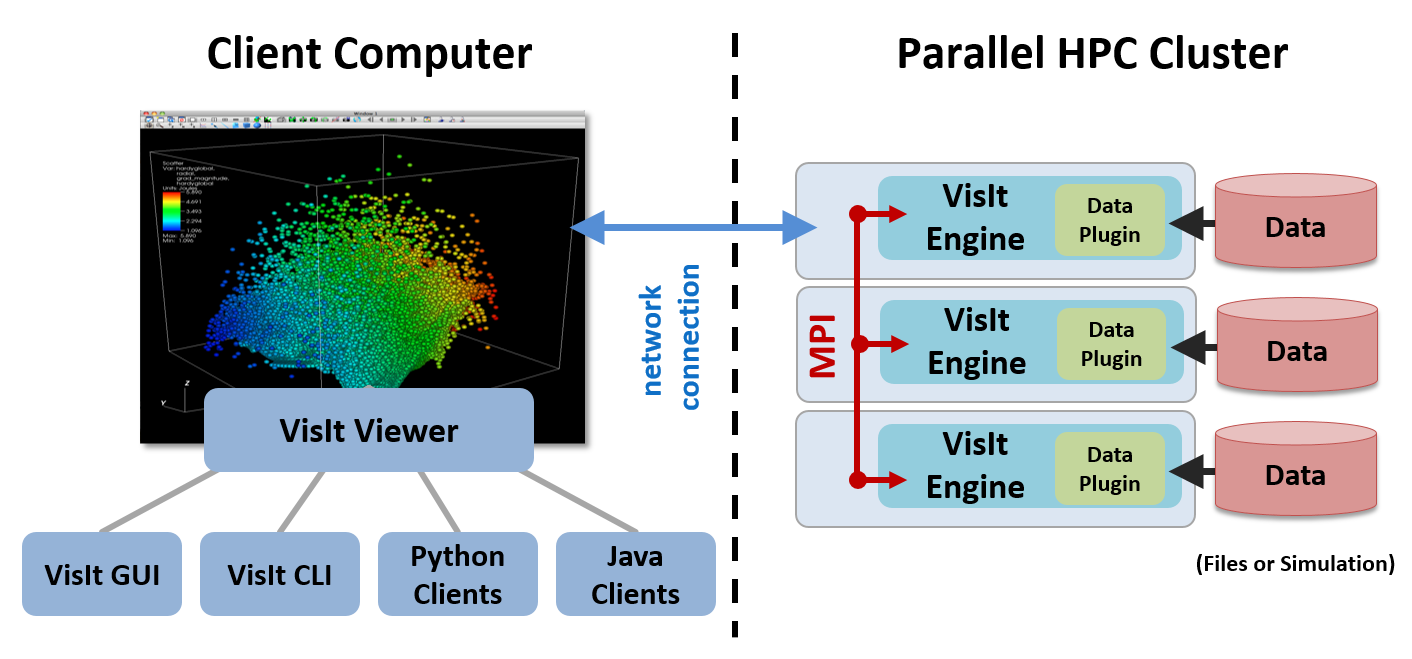
\includegraphics[scale=0.5]{figures/Visit-Architecture.png}
\caption{VisIt architecture showing client connected to the viewer, with remote engines on the HPC platform running within an MPI communicator. Since we are interested in in situ workflows, we suppose that the data is gotten from a running simulation rather than files, (Figure from~\cite{noauthor_visit_works}).}
\label{figvisit}
\end{figure}

We also find several tools that were meant for IO management and then adapted for in situ analytics. ADIOS1\cite{lofstead_insights_2013_adios, jin2008adaptive_adios, boyuka_transparent_2014_adios, in_situ_methodes} and Damaris\cite{dorier_damaris_2012} 
are examples of frameworks in that category. FlowVR\cite{dreher_flexible_2014} on its side was developed for virtual reality and has been adapted to support both in situ and in transit analytics.

The Adaptable Input Output System (ADIOS) is a middleware that provides a generic interface to use transparently different IO transport layers and data handlers.
It has a set of built-in IO systems, including HDF5, NetCDF, POSIX, and MPI-IO.
ADIOS is configurable through an XML file where one can describe the data and select a library to handle it (write, read, or process) outside of the running simulation. 
FlexIO~\cite{zheng_flexio_nodate} is an example of in situ tools built on ADIOS. It is a middleware for coupling simulations with in situ analytics in ways that offer placement flexibility to those online analytics and visualization codes. 

ADIOS2,  the second generation of ADIOS, supports in situ processing as a built-in functionality thanks to the  Sustainable Staging Transport engine (SST) that allows a direct connection between the simulations and the in situ processing codes. The SST buffers and sends the requested data over network using the same ADIOS write/read API as the file-based IO systems. The in situ workflows in ADIOS2 are set up similarly to IO workflows through the XML configuration file~\cite{laufer2022high_adios2_insitu}.

Damaris\cite{dorier_damaris_2012, dorier_damaris_2012_tech_report} is another library that was designed originally for IO and then used for in situ processing. Damaris leverages helper cores and shared memory to reduce the IO jitter. It usually dedicates one core per node for IO operation, which is called a \textit{server}. 
Damaris is a set of MPI processes running on a set of dedicated cores(severs). Just like ADIOS, Damaris uses an external file for configuration. In~\cite{dorier_addressing_2014, dorier_lessons_2015, dorier_damaris, damaris_viz} Dorier \textit{et al.} use Damaris for in situ analyics. They keep the data in shared memory segments and perform in situ analytics and visualizations, filtering, indexing, and finally, IO in response to user-defined events sent either by the simulation or by external tools.  

FlowVR~\cite{allard_flowvr_2004, allard_distributed_2006_flowvr, arcila_flowvr_2006} is a middleware dedicated to virtual reality (VR) that is built on the dataflow\cite{sousa2012dataflow} paradigm and has been used for scientific visualization. 
An application in FlowVR is composed of modules exchanging data through the network. A module is a code that has been augmented with FlowVR methods. There is no explicit dependency between modules; they only exchange data with a daemon that runs on the same host. Once modules are defined, they are assembled, connecting their input and output ports. The application is thus represented as a dataflow where nodes are the modules, and the edges are First In First Out (FIFO) communication channels.
With its dataflow architecture, FlowVR has been explored for in situ, in transit, and heterogeneous workflows in the work of M. Dreher \textit{et al.}~\cite{dreher_methodes_2015, dreher_flexible_2014, dreher_exavis}. 


Due to its efficiency, in situ processing emerged quickly for general-purpose usage rather than focusing on specific tasks and visualization. Sensei~\cite{ayachit_sensei_2016, bethel_sensei_2022, noauthor_sensei_web, git_sensei_2022}, a generic in situ interface that focuses on having a unified API to instrument the simulation codes and making use of several external tools to handle data like Libsim, Catalyst, or user-defined analysis codes. 
Its architecture is built on three main components: a data adaptor to map simulation data to the VTK data model, an analysis adaptor to map the VTK data model to the model used on the analytics side, and a bridge to link the two adaptors and provide the methods called by the simulation to trigger in situ analytics. The bridge can be the VTK data model itself. Sensei already supports several backends, such as Alpine/Ascent/VTK-m\cite{Larsen-alpine-isav17, moreland_vtk-m_2016}, ADIOS\cite{lofstead_insights_2013_adios, boyuka_transparent_2014_adios} as well as for Paraview/Catalyst and VisIt/Libsim. Figure~\ref{figsensei} shows a schematic architecture of Sensei. 

\begin{figure}[tb]\centering
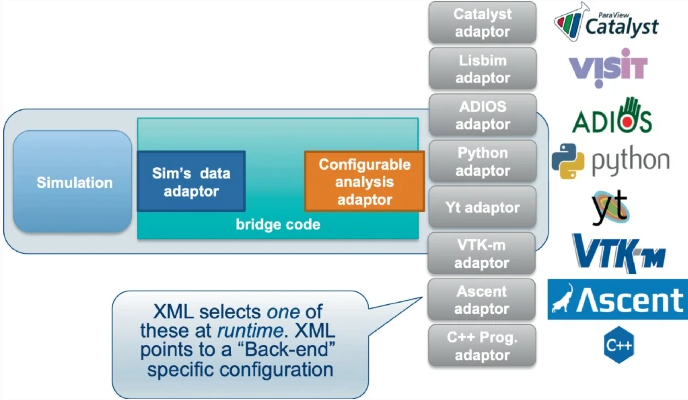
\includegraphics[scale=0.5]{figures/sensei.png}
\caption{Sensei architecture showing a single data producer that has access to any number of potential in situ or in transit methods. The runtime choice, along with its associated parameters, is specified in an XML configuration file, (Figure from~\cite{bethel_sensei_2022}).}
\label{figsensei}
\end{figure}

Ascent\cite{ noauthor_ascent_nodate, Larsen-alpine-isav17, triggers_ascent, Larsen_ascent} is a lightweight in situ library that is designed to run in the same resources as the simulation. It integrates with many technologies (ADIOS, Babel Flow \cite{babel}, ParaView/Catalyst and Python), supports both visualization and analysis routines, and provides support for modern supercomputers~\cite{childs2022situ}.  
It uses conduit~\cite{larsen_strawman_2015, noauthor_conduit_nodate} as a bridging data model between the simulations and the supported backends that simplifies describing hierarchical scientific data. It also implements VTK-h, to add a distributed memory layer to VTK-m, which already minimizes memory usage and execution time, to support both efficient shared and distributed memory configurations. 

SmartSim\cite{smartsim_2022, site_introduction_smartsim, partee2021using_smartsim} is a library dedicated to enabling in situ analysis and machine learning (ML) for traditional HPC simulations. It provides a different way to couple simulations with analytics, by using the Redis\cite{redis} in-memory key-value store~\cite{idreos2019learning_key_value}. 
The Smartsim architecture is built on two main components: the SmartSim Infrastructure Library (IL) and SmartRedis. The first is a python-based workflow library that launches in-memory storage alongside HPC applications and facilitates the dynamic execution of simulations and ML infrastructure. 
The second consists of a lightweight client library used in applications to communicate with infrastructure launched by SmartSim. 
The data generated by the simulation by the clients into the Redis in-memory store. Then the SmartSim IL gets the data from the store and uses them to feed the ML models.

Decaf\cite{dreher_decaf_2017}, a dataflow middleware for in situ workflows. Similarly to FlowVR, Decaf composes multiple executables to form a workflow. However, it does not rely on a separate daemon to manage the graph execution. A Decaf workflow is composed of several dataflows. Each dataflow is the association of a producer, a consumer, and a communication object called a \textit{link}.  The \textit{link} is deployed in a set of separate resources where operation on the data structure can be performed. Bredala\cite{dreher_bredala_2016} is built on Decaf; it provides an API to construct a data model with enough information to keep its semantics while splitting and merging. The work on Decaf and Bredala was a strong base to propose a new concept to automatically extract needed data for analytics at the producer, called contracts\cite{mommessin_automatic_2017}.


DataSpaces~\cite{docan_dataspaces_2012} is a distributed virtual shared memory space implemented on staging nodes. 
In a client/server fashion where the running simulations are clients, and DataSpaces nodes are servers.  
The goal of DataSpaces is to enable the data of interest, which is extracted from a running application, to be efficiently indexed and asynchronously accessed and processed by other components in the simulation workflow. 
Data extraction is performed by the Decoupled and Asynchronous Remote Transfers (DART) library~\cite{DART_2008, docan2010enabling_dart}. 
DART is built on Remote Direct Memory Access (RDMA) technology to enable fast, low-overhead and asynchronous access to data from a running simulation, and support high-throughput, low-latency data transfers~\cite{bennett_combining_2012_dataspaces}. 
DataSpaces extends existing parallel programming models, such as MPI and Partitioned Global Address Space (PGAS), with a simple set of APIs. In order to enable the coupling of workflow component applications, DataSpaces provides the \texttt{put}/\texttt{get} operators to access the virtual shared store. As already mentioned DataSpaces servers are launched in staging nodes, thus it enables in transit workflow configurations rather than in situ.

Wu \textit{et al.} in~\cite{wu_diva_2020} propose a declarative and reactive language and runtime for in situ visualization called DIVA that can extend existing in situ systems such as VTK. DEIVA is built on MPI and consists of two main components: functional reactive programming (FRP) visualization-specific language and a low-level C++ dataflow API. FRP\cite{ wan2000functional_FRP, blackheath2016functional_FRP, perez2016functional_FRP} is a programming paradigm that describes systems that operate on time-varying data, which is well adapted for in situ visualization purposes. The users describe their codes using the declarative API. Then the language parser translates it into an internal DAG. This last is finally interpreted then to the low-level C++ dataflow API for execution. DIVA language does not support directly in transit workflows.
 
\subsubsection{Discussion}
In this section, we have presented a set of in situ tools, ranging from visualization and AI-specific to general-purpose in situ workflow management systems. 
We had a variety of tools that could be classified according to multiple axes. For instance, ParaView Catalyst, and VisIt Libsim are synchronous, whereas the other presented tools may run asynchronous analytics too. One can compare how in situ analytics are coupled to the simulation, either embedded in the code or less intrusive such as in FlowVR and DataSpaces, where simulations are not aware of other applications. The data model is also different. Several tools are based on VTK or support it (ParaView Catalyst, VisIt Libsim, ADIOS, Sensei and Ascent), SmartSim uses Redis in-memory store, and Bredala implements its own data model. The in situ workflows may be statically generated and configured, or in situ tasks may be created in response to specific events. For instance, Decaf or FlowVR workflows are created with a static configuration where we know a priori the producer and the consumer that we link together, unlike DataSpaces and SmartSim, where the clients may request analytics tasks as moving on.  

Despite all these differences, most of those tools share a common specification which is relying on static parallelization.
Mapping the analysis workflow tasks to compute resources statically often leads to high performance but requires the user to control this mapping explicitly. The underlying transport layer is often based on MPI %(except for SmartSim, which is based on tcp~\cite{site_introduction_smartsim}, FlowVR and ADIOS) 
which simplifies the coupling with the simulations, but may imply rewriting the parallel in situ analytics with MPI too, which is very complicated for the reasons we have already mentioned in Section~\ref{sec:discussion:programmingmodels}.

 
\subsection{Task-based Programming for In Situ Workflows}\label{sec:insitu:taskbased}

In this section, we will have a look at the use of the task-based programming model in the in situ workflows and discuss the reasons why we need to work more on this topic.

Task-based programming in shared memory is commonly used today in scientific applications to efficiently leverage nodes architecture, using OpenMP\cite{openMP} or Intel OneAPI Threading Building Blocks (TBB)\cite{Robison2011tbb}. In addition to eventual embedded in situ routines in the simulation codes, both libraries have been used in standalone in situ tools. 

GoldRush\cite{zheng2013goldrush} is an in situ technique that exploits idle node resources for in situ data analytics. It is built on ADIOS IO system and FlexIO transport, already presented in section\ref{sec:insitu:tools}. Unlike other in situ methods, GoldRush detects when the simulation does not use all available cores to launch in situ tasks in idle threads as long as there is enough memory. Typically this is possible within non-parallelized computations, MPI communications, and file IOs. At the end of an OpenMP region, a SIGCONT signal is emitted to start in situ analytics, and a SIGSTOP signal stops it when the simulation reaches the next OpenMP parallel region. 
This approach has several benefits, including the efficient use of compute node resources and reductions in data movement overheads.

TBB library provides a task-based programming model and a work-stealing scheduler for shared memory. It has been used in TINS\cite{yokota_tins_2018, dirand2018integration} for in situ analytics. In this work, both simulation and analytics are task-based, and TBB is used to dynamically distribute the simulation and the analytics tasks to the available cores. Even if TINS and GoldRucsh use similar approaches, they act on two different levels: TINS at the task level and GoldRush at the system level. TINS has been compared to both GoldRush and Damaris with static and dynamic helper core strategies in  ~\cite{dirand2018tins}, and the results show that TINS outperforms both tools.

Task-based programming has been used in an in transit configuration in Sun \textit{et al.} paper~\cite{staging_2016_manish}. The proposed work is built on the DataSpaces system. It proposes an asynchronous coupling of distributed task-based scientific workflow where both simulation and in situ analytics are parallelized in a task-based fashion. 

\subsubsection{Discussion}
In this section, we have focused on the usage of task-based programming for in situ workflows. The utilization is restricted to shared memory with TINS and GoldRush in addition to eventual embedded in situ routines in simulation codes. 
The only attempt to use task-based programming for in transit analytics was in Sun \textit{et al.} paper, where both the simulation and the analytics were parallelized in tasks. 

To our knowledge, there is no work trying to couple distributed task-based programming with MPI for in situ/in transit analytics.
Shared memory task-based models are usually easy to couple with other programming models, such as MPI. As their utilization is encapsulated in one MPI process, (like if it was just a sequential program), which does not create integration complexity or incompatibilities between the two models' concepts.  
Consequently, using them does not raise the same challenges as coupling distributed task-based programming with MPI, which we will discuss in Chapter~\ref{chap:approach}.


\subsection{Big Data Frameworks for In Situ Workflows}\label{sec:insitu:bigdata}

In this section, we present the attempts to use big data frameworks for in situ analytics.  

Big Data models are built on several other programming models such as functional, SQL-based, and Actor models. The current defacto framework/model for writing data-centric applications is Map-reduce~\cite{Wu2017}.
SMART~\cite{wang_smart_2015} (inSitu MApReduce liTe) proposes a Map-reduce~\cite{dean2008mapreduce} interface for programming in situ analysis on top of MPI/OpenMP. 
A Map-Reduce program is composed of a map and reduce procedures. The map method performs filtering and sorting, and the reduce method performs a summary operation. 
SMART supports a variety of scientific analytics on simulation nodes, with minimal modification of simulation code. It supports efficient in situ processing by accessing simulated data directly from memory in each node of a cluster or a distributed memory parallel machine. SMART is the first in situ framework based on a Map-reduce-like model.


Paper~\cite{zanuz_-transit_2018_flink} appeared in 2018 and uses another big data tool in in situ workflows. It takes benefit of Flink~\cite{carbone2015apache_flink, friedman2016introduction_flink} stream processing support for enabling in transit analysis.
The architecture of the proposed framework connects the 
simulation parallelized with MPI to Flink worker nodes using ZeroMQ~\cite{hintjens2013zeromq}. Flink executes the analysis scripts in parallel, then injects results to the HBase distributed database~\cite{vora2011hadoop}, which takes care of storing the results using its local disks. 
The model provides a loose control on data partitioning that is not well adapted to support efficient parallelization of patterns such as stencil computations\cite{arrayUDF-SC2018} or large-scale linear algebra.

%The tentative of using big data frameworks for in situ processing is quite similar to our work in a high-level view. That is to couple big data tools with MPI. The issue with those tools is that they are not either the most adapted tools for scientific data processing.   


\section{Distributed Task-based Frameworks}\label{sec:task-based-frameworks}

Distributed task-based model alongside Pythonic programming are gaining more and more popularity for the intuitive programming interface and orchestration they provide together. In this section, we present some of those systems and highlight their differences.  

Parallel Scripting Library (Parsl)~\cite{babuji2017introducing, babuji2018parsl, babuji_parsl_2019} is a pythonic scripting library that can express parallelism between both Python code and components written in other languages. Parsl uses \texttt{Apps} decorators to intercept and modify the behaviour of Python functions: the \texttt{@python\_app} decorator is used for pure Python functions and \texttt{@bash\_app} decorator for shell commands. When \texttt{App} decorator is invoked, an asynchronous task is registered, and a \texttt{Future} object is returned immediately. \texttt{Futures} can be passed as an argument to \texttt{App}, indicating a dependency between the two tasks. 
Parsl runtime manages the execution of the parcel-annotated programs on the configured resources by creating a dynamic task graph, where nodes are programs (tasks) and edges are the input/outputs exchanged between tasks. The data can be any serializable Python object, files or \texttt{Futures}. 
 Parsl provides several executors, depending on applications, which allows running those tasks on one or more target execution resources. Figure~\ref{figparsl} shows how Parsl programs are transformed into DAGs and then run in the executors.  

\begin{figure}[tb]\centering
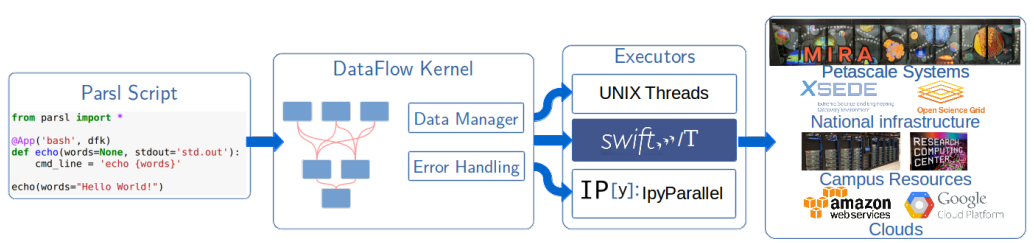
\includegraphics[scale=0.44]{figures/parsl.png}
\caption{Parsl architecture: DataFlow Kernel (DFK) maps parsl-annotated scripts to Executors that support diverse computational platforms~\cite{babuji2018parsl}.}
\label{figparsl}
\end{figure}


Writing parallel programs in Legion\cite{bauer_legion_2012} needs both programs to be expressed in terms of \texttt{Tasks} and data into \texttt{Regions} to be distributed across several machines. Logical regions are the fundamental abstraction used for describing program data in Legion applications. 
Pygion\cite{slaughter_pygion_2019} is the Python high-level interface of Legion. Here again, Python decorators are used to mark functions for parallel execution. A program is divided into several tasks using \texttt{@task} to be executed in parallel and program data into \texttt{Regions} and \texttt{Subregions} to express data parallelism. 
The arguments to \texttt{Tasks}, and the \texttt{privileges} requested on those arguments (read, write, etc.) are used to compute a dependency graph between tasks that guides the parallel and distributed execution of the program. There are also dependencies between two tasks if they access overlapping data, and at least one of the tasks wants to write in that region.  
Early experiments for in situ visualization subsystem were prototyped using Legion in~\cite{heirich2017situ}.  
It shows Legion runtime manages to interleave simulation and visualization tasks without reducing the simulation throughput. However, using the implemented tool requires code modifications to redesign an MPI+X application into a Legion.

Several other interesting task-based frameworks are found in the literature. For instance,  
StarPU~\cite{augonnet2009starpu, augonnet2010starpu, archipoff2017starpu} is a runtime system for scheduling a graph of tasks onto a heterogeneous set of processing units. It provides a unified execution model and data management library for heterogeneous systems.
Parallel Runtime Scheduling and Execution Controller (PaRSEC)~\cite{bosilca2013parsec, hoque2017dynamic} is a task-based runtime for distributed architectures capable of tracking and moving data from different nodes. Dependencies between tasks are explicitly described, and the task graph is generated automatically from a domain-specific language (DSL). These approaches can improve usability within a domain as long as the target programs are well supported by the domain-specific semantics~\cite{slaughter_pygion_2019}. In addition to the DSLs, PaRSEC runtime has several components namely: schedulers, communication engines and data interfaces. 
Despite the similarities between Those tools, only Pygion supports data partitioning~\cite{treichler2016dependent_partitioning} through \texttt{subregions}; the others require users to reorganize data in applications that use multiple access patterns explicitly. 


PyCOMPSs\cite{tejedor2017pycompss, ramoncortes_programming_2020_pycompss} is the Python binding of the COMPSs\cite{tejedor_compss} task-based system. 
%It has been developed with the reflection that Python has a lot of advantages (free, compact, readable, very suited for rapid prototyping, a rich set of scientific libraries, integration with lower-level languages: C/C++, etc.), but it has to target distributed platforms to be used in larger projects. 
Similarly to Parsl and Pygion, the user has to identify the task that may be run in parallel and annotate them using decorators. And then a runtime system analyses the script to identify the dependencies between those tasks depending on the arguments of the \texttt{@task} decorator. Among other arguments, there are the parameters of the decorated function, whose name is the formal parameter’s name and whose value defines the type and direction of the parameter. Those arguments are needed to construct the dependency graph. 
PyCOMPSs added support to a distributed data structure, namely \textit{ds-array}~\cite{cidfuentes_dislib_2019_pycompss} that offers a parallel and almost the same API as NumPy\footnote{https://numpy.org/}. 
It also supports MPI programs~\cite{elshazly_performance_2020_pycompss} as tasks to be integrated into the task graph. 
PyCOMPSs is part of the eFlow4HPC\footnote{https://eflows4hpc.eu/} project to provide HPC workflows as a service. It allows streaming communication between different parts of a workflow that can be used to evaluate intermediate results and enables the implementation of in situ optimization algorithms~\cite{ejarque_enabling_2022}. 

Until now, an MPI application can be integrated into PyCOMPSs as a task. In other words, the MPI applications are encapsulated into tasks, so they are started when the task is launched and once they are finished they share the produced data with that task, which is another possible way to couple MPI with task-based programming.

In the context of Parallel libraries, \dask~\cite{rocklin_dask_2015} is one of the most interesting task-based Python frameworks because it offers access to parallel versions of well-known libraries such as NumPy and Pandas\footnote{https://pandas.pydata.org/} with \texttt{dask.array} and \texttt{dask.dataframe}, respectively. 
Those two alongside \texttt{dask.bags} are called collections. It also provides a parallel version of Scikit-learn\footnote{https://scikit-learn.org/stable/} called \texttt{dask\_ml}. 
\dask is able to construct task graphs automatically thanks to blocked algorithms, that resolve small problems to compute a larger one. For instance, in order to compute the sum of a large array, we can compute the sum of smaller blocks and sum all intermediate sums.
In addition to those high-level collections, there is also a possibility to construct the graph manually using a lower-level API using \texttt{Futures} and decorated functions. 

Ray~\cite{222605_ray}, another well-known task-based framework, has a distributed scheduler.
It is used to scale both artificial intelligence (AI) and python applications. The system architecture can be structured into two main components: the Ray core, which enables scalable applications to be built in pure python, and Ray AIR~\cite{noauthor_ray_AIR_nodate}, which provides several libraries (\textit{Datasets} for distributed data preprocessing, \textit{RLlib} for Reinforcement Learning~\cite{liang2018rllib}, \textit{Tune} for scalable hyperparameter tuning\cite{liaw2018tune} and others) that enables simple scaling of AI workloads \cite{noauthor_ray_nodate}.   
Ray provides a scheduler for \dask: \dask\_on\_ray\cite{noauthor_using_nodate}. This takes advantage of both frameworks: \dask collections to write analytics using familiar APIs and Ray-specific features such as the distributed scheduler, shared-memory store and others.  
Ray is less mature compared to \dask and does not have built-in primitives for partitioned data. However, it is more suited for heavy workloads and AI where it has been shown that it outperforms \dask~\cite{puurula_benchmarking_2019}.

An interesting taxonomy of task-based programming models with recommendations is already done in~\cite{gurhe2021}. 

\subsection{Discussion}\label{discussionTaskBased}
In this section, we have presented some of the well-known distributed task-based frameworks. We tried to pick the most relevant to our work either for their ease of use, related tentative for in situ usage or coupling with MPI applications. 

Each of the presented frameworks has interesting features that make it relevant to specific needs. For instance, 
Parsl is a good candidate for general-purpose usage thanks to the different executors it offers. 
Legion has the particularity of being able to express data parallelism in addition to tasks which makes it more interesting to use in data-driven workflows. 
PaRSEC generates its task graph from a DSL which is an interesting approach too because it takes advantage of the dynamicity of task-based programming at a low level and the abstraction level of DSL at a higher level. 
PaRSEC scheme is very interesting as it could be used for domain-specific in situ analytics, coupled with MPI simulations. Such configuration would be relevant for domain scientists that are used for DSL usage. The issue with such a scheme is the need for the development of new task-based DSLs.
PyCOMPSs and other development in the eFlow4HPC is also interesting as it considers providing HPC workflows as a service, which would likely hide all coupling complexity and allows using PyCOMPSs to write task-based in situ analytics, but for the moment, no work has been published on this topic. 
From the user API perspective, \dask seems to be the most relevant thanks to the provided distributed libraries, which allow writing  almost sequential python codes that run in parallel.  Ray on its side may be the best tool for AI workloads as it provides both interesting API and performance compared to \dask.

The rest of this discussion is driven by two main aspects: coupling distributed task-based frameworks with MPI, and the most relevant tool to use for in situ processing among all cited examples.
First, there were relevant attempts to couple distributed task-based tools with MPI: 
in PyCOMPSs~\cite{elshazly_performance_2020_pycompss}, an MPI application can be launched in a PyCOMPSs task. This is a way to perform the coupling. However, it is not possible to use it in our case for several reasons: 
first, in our work, we consider scientific applications that generate huge amounts of data; launching them within a task and then gathering the results in the same node may not be possible for memory reasons. The second issue is that scientific applications are usually iterative; it is not possible to extract the data at each timestep from a task (to perform in situ analytics) and keep it running. This violates the definition of a task. Note that we want to simplify writing in situ analytics using distributed task-based frameworks while keeping the MPI simulation as is, so we don't consider rewriting those simulations in other paradigms.  

Another attempt was to use MPI with \dask in~\cite{shafi_efficient_2021}, but it was as a transport layer rather than coupling with MPI programs. Mainly, in this work, the authors have added a new implementation using MPI to the already-used RPC communication system to replace TCP or UCX. This work can be considered to optimize a solution based on \dask to unify the transport layer between simulations and analytics written in \dask. 

The second aspect is to pick the most relevant tool to use for in situ processing, and this time, from the user perspective. 
We want to propose a solution that minimizes the changes in the existing post hoc analytics codes to work in situ and to facilitate the development of new ones.   
Given that Python is the most used language for data analytics, pythonic tools are more advantageous, but it is not enough, as most of the presented tools are. 
The interesting aspect to consider is the available distributed APIs to write analytics and whether they are similar to sequential Python APIs, which scientists were used to to write post hoc analytics. And here, PyCOMPSs and \dask already provide parallel versions of some known libraries, which makes them more favourable. 

\section{Summary}
In this Chapter, we have defined our context and discussion the related work to our topic.
We have defined high-performance computing and justified the need for it to solve complex problems. 
We have presented two of the programming models: message passing and distributed task programming, which are used to program those huge machines, and then we raised the IO bottleneck issue that faces large-scale simulations in domains such as nuclear fusion. 
We have presented two analytics workflows used to process the data generated by HPC simulations, namely: post hoc and in situ workflows. 
The first suffers from the IO bottleneck, and the second is quite complicated to set up.

Our goal is then to provide a solution that brings together the in situ performance and the post hoc ease of use. Thus in the second part, the related work, we have mainly two topics. 
The first presents and discusses the existing in situ tools, how they work and their specificity, and eventual attempts to use task-based programming or other big data models for in situ analytics. 
The second presents task-based frameworks and where they have been used for in situ analytics or at least coupled with message-passing programs. 


\chapter{Used Tools}\label{chap:tools}

\vspace{20mm}
\epigraph{\textit{If I have seen further than others, it is by standing upon the shoulders of giants.}} {Isaac Newton}

\vfill

Now that we have had a look at some of the existing in situ platforms and tools and have an idea about the emergence of distributed task-based programming in big data and some attempts at using it for in situ analytics, we are going to present the tools we will use in this work.

we have opted for \dask distributed to use as a task-based framework for in situ analytics. This choice has been motivated by the ease of use of \dask, from the user perspective, and we target a more general-purpose tool rather than a specialized one.

In addition, we have chosen to provide a clean solution that separates concerns, namely the physics under study and the way we handle data. We have opted for \pdi data interface as a data handler ( which is developed in Maison de la Simulation). It is used in multiple production codes such as Gysela\footnote{https://gyselax.github.io/}, ARK\footnote{https://gitlab.erc-atmo.eu/erc-atmo/ark}, Alya\footnote{https://compbiomedeu.github.io/applications/Alya/Alya.html} and GYM-DSSAT\footnote{https://rgautron.gitlabpages.inria.fr/gym-dssat-docs/}.


\newpage

\section{\dask Distributed}\label{sec:dask.distributed}

In this section, we will present the \dask distributed framework and how it operates internally. 
When we started working on the project, the documentation regarding the scheduling, the internals and how the \dask distributed operates and manages tasks internally, and the different actors were not as developed as they are today\cite{noauthor_daskdistributed_nodate}. 
So most of the concepts that are presented are coming mostly from the paper\cite{rocklin_dask_2015}, \dask GitHub repository code\cite{amal_distributed_2022}.

\subsection{Overview}

\dask is a Python framework that enables parallel and out-of-core computations. This work is based on the distributed version of \dask, named \dask Distributed because our goal is to perform in situ analytics for large-scale distributed simulations.
By abuse of language, we will say \dask instead of \dask Distributed in the rest of this document. 

\dask is built on the client/server scheme. 
It has three main components: one or more \textit{clients}, a \textit{scheduler}, and one or more \textit{workers}, as shown in Figure~\ref{figdaskarchi}. 
The client is the entry point to the \dask cluster; it represents an interface between the end-user and \dask. It submits analytics to the scheduler as a task graph. 
The scheduler analyses the task graph and checks for any connected workers; if so, it sends the ready tasks to the idle workers. The workers are multi-threaded processes that perform the computations and store or share the data.
The source of the data in \dask is usually a storage system.

The code in Listing~\ref{listdask} is typical client code in a \dask workflow. It runs following these steps that are also represented in Figure~\ref{figdaskarchi}: 
the client first connects to the scheduler. 
It reads the metadata of the HDF5 file \texttt{"data.hdf5"} from the parallel file system. 
A \texttt{dask.array} object is created from the descriptor returned in the previous step. 
The \texttt{mean()} method and the multiplication operation create a task graph that is submitted to the scheduler by the call to \texttt{compute()}. The task graph generated by Listing~\ref{listdask} is shown in Figure~\ref{figtaskmean}. 

The scheduler then sends it to the workers as they become ready. 
The first ready tasks are \texttt{getitem} tasks that read data from the file.  
Note that it is at this stage (when tasks are sent to the workers) that the data is read from the file system, which makes it possible to process data larger than the memory of one node in parallel.
Once all the tasks are computed, the result is returned to the client.

Listing~\ref{listnumpy} represents a typical python analysis without \dask; Listing~\ref {listdask} illustrates a \dask parallel equivalent. 

\begin{lstlisting}[float=h!, label=listnumpy, language=python, caption=Sequential post hoc mean using numpy]
import numpy as np
import h5py
# Load data from HDF5
data = h5py.File('data.hdf5',mode='r')['dataset1']
# Compute the mean of the array
computed_mean = np.array(data).mean()*200
print("Computed mean : ", computed_mean)
\end{lstlisting}

\begin{lstlisting}[ float=h!, label=listdask, language=python, caption=Parallel post hoc mean with \dask. Lines differing from the analysis of Listing~\ref{listnumpy} are highlighted]
|\hlline|import dask.array as da
import h5py
|\hlline|# Connect to Dask
|\hlline|client = dask.distributed.Client(address)
# Build a lazy array descriptor from HDF5
data = h5py.File('data.hdf5',mode='r')['dataset1']|\label{post:hdf5}|
|\hlline|daskdata = da.from_array(data, chunks=(1, 5, 5))|\label{post:chunk}|
mean = daskdata.mean()*200
|\hlline|computed_mean = mean.compute()
print("Computed mean : ", computed_mean)
\end{lstlisting}

\begin{figure}[ht!]\centering
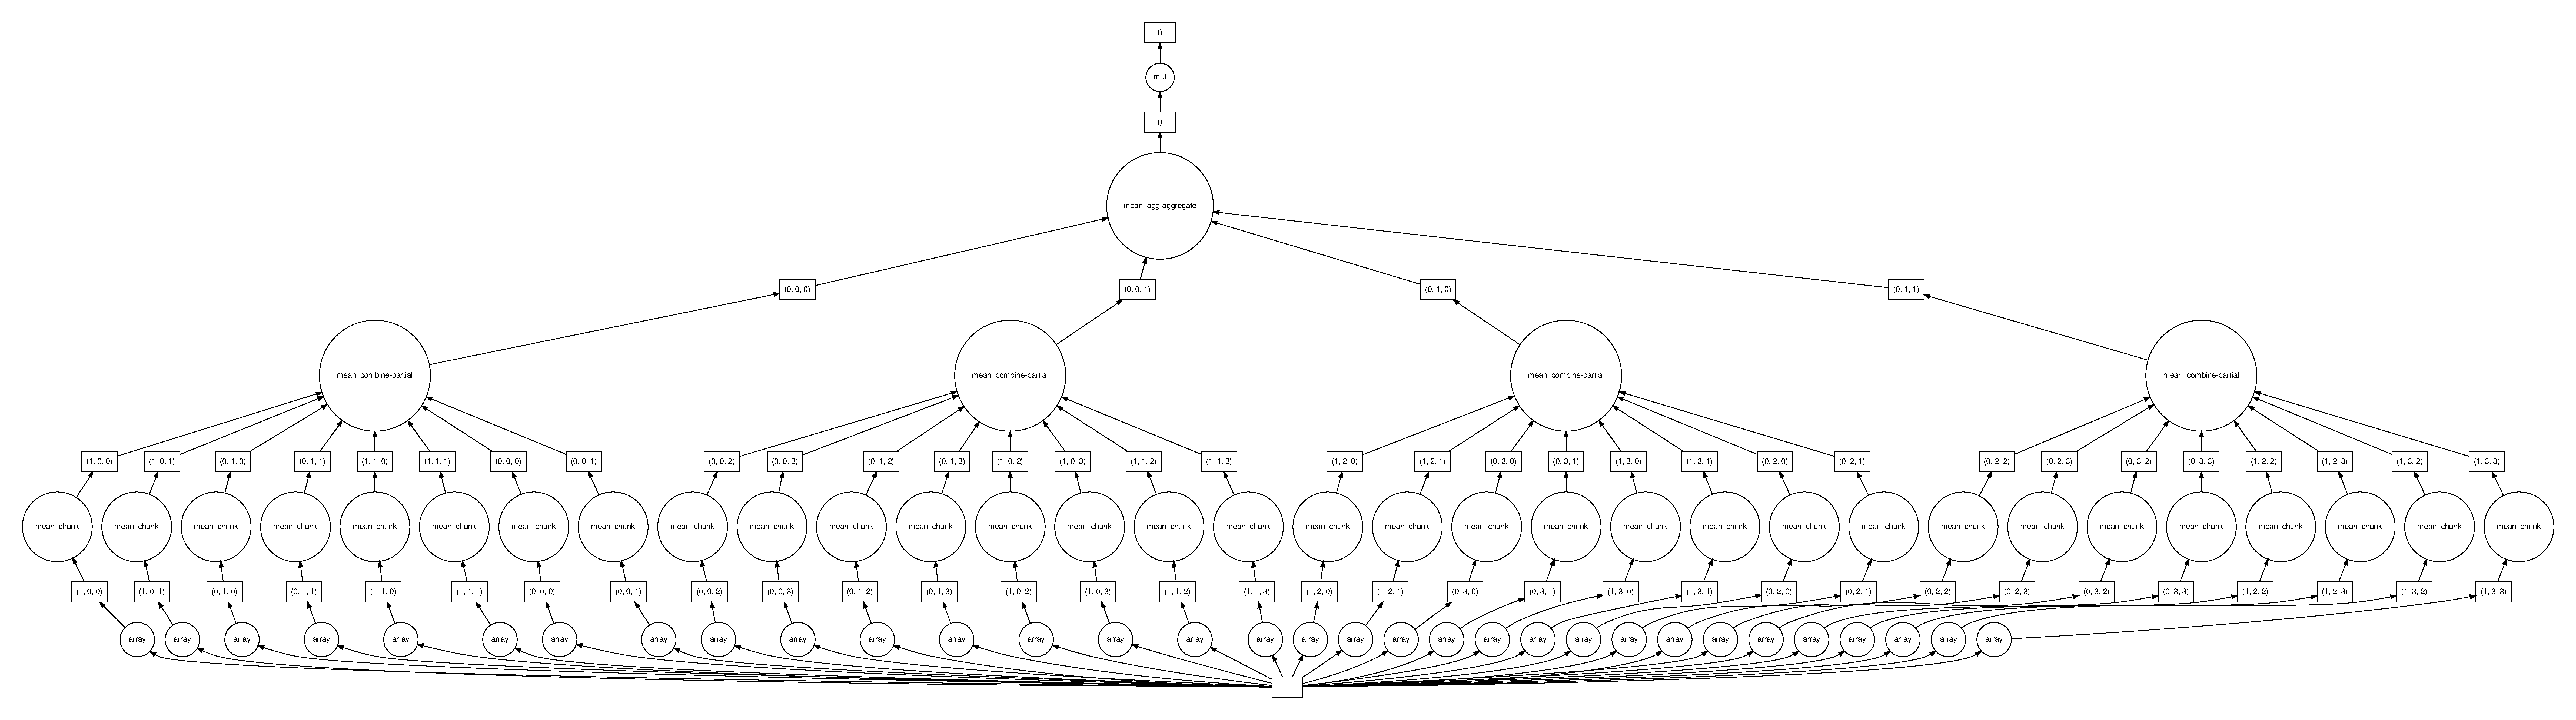
\includegraphics[scale=0.145, angle=90]{figures/mean.pdf}
\caption{\dask graph generated in Listing~\ref{listdask}. The HDF5 dataset size is $(2, 20, 20)$ and chunk size is $(1, 5, 5)$. From the bottom to the top of the graph, we have `array` tasks that correspond to reading the chunks from the file, followed by local `mean` computations and then the `mean` aggregations. And finally, a `mul` operation corresponds to `*200` in the script.}
\label{figtaskmean}
\end{figure}

\begin{figure}[tb]\centering
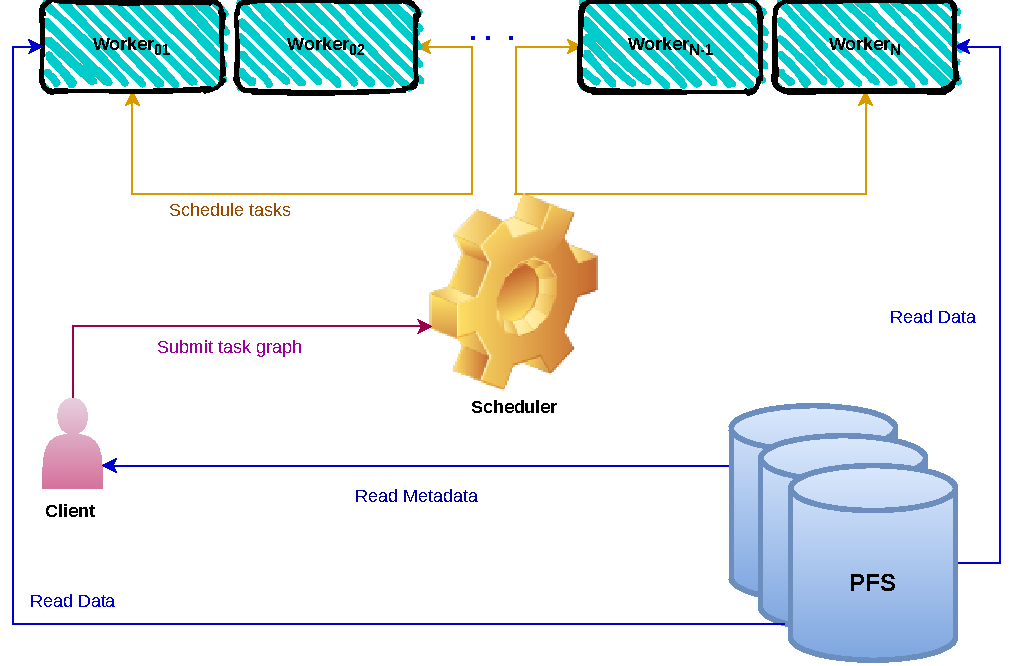
\includegraphics[scale=0.6]{figures/DaskArchiecture.pdf}
\caption{\dask distributed architecture in a typical post hoc workflow. A client and $N$ workers are connected to the scheduler. 1) The client reads small metadata regarding the needed files from the PFS, 2) creates the \dask data structure and submits a task graph, 3) the workers execute the tasks, 4) some of them read data blocks in parallel from the PFS.}
\label{figdaskarchi}
\end{figure}

\subsection{Tasks in \dask Distributed}\label{sec:task}

The tasks are a central concept in \dask and all task-based frameworks; it is the smallest piece of work that can be submitted to the scheduler and run by a worker. 

In this part, we detail how \dask handles and implements this concept, starting with task graph creation, the task state transition, and finally, task scheduling. 
We define and discuss \textit{pure data tasks} and how they are used in our work. Alongside those important low-level details, we present \dask collections that will strengthen our choice by showing the ease of use of \dask and its underlying submodules.  

\subsubsection{Task Graph}\label{sec:taskgraph}

Every script submitted to \dask scheduler is first translated to a task graph, specifically a directed acyclic graph of tasks with data dependencies. 
The \textit{graph} is represented as a dictionary, where the keys (identifiers) are any hashable value that is not a task, and the values are computations. 
A \textit{computation} can be a key present in the graph, a value such as an integer, a task, or a list of computations. 
A \textit{task} is described in the dictionary as a Python tuple that has a callable as a first element, such as a function or an object of a class that implements the \textit{\_\_call\_\_()} magic method; followed by a list of arguments, and an argument may be any valid computation.
For instance \texttt{(function1, arg1, arg2, arg3)} is a task that applies \texttt{function1} to \texttt{(arg1, arg2, arg3)} where the arguments are valid computations such as: \texttt{{arg1: 1, arg2: (function2, arg4), arg3: [(function3, arg5, 0.2), 5]}}.

When executing the task described by \texttt{(function1, arg1, arg2, arg3)} in the dictionary, the worker runs \texttt{function1(arg1, arg2, arg3)}, by moving the opening parenthesis one term to the left, the execution of \texttt{function1} is delayed. This representation allows \dask to store this computation as data that can be analyzed by the scheduler later rather than cause immediate execution.   

The user can use the \texttt{Delayed} API to customize and create his own task graph. It may be advantageous when the user has particular processing which is not covered by the high-level collections. 
Moreover, \dask implements a \texttt{future} API, which is immediate rather than lazy. 

Listing~\ref{listdelayed} shows an example of task graph creation in \dask using the low-level \texttt{Delayed} decorator. The created task graph is shown in Figure~\ref{figfunc}. 
We use the \texttt{delayed} decorator to declare lazy functions to \dask scheduler, and then we use them to create a task graph. 
It is represented as a dictionary (Line\ref{linedict}) where we can see the keys generated by \dask, the functions and the arguments, for instance: \texttt{'func-f0310b3c-f9ed-4199-b3bb-dda81384823a': (<function \_\_main\_\_.func(a, b)>}, \texttt{'add-e11deea3-1568-4abf-9ae5-a6491a7f46d8'}, \texttt{'product-e7451475-cfe2-4ae5-9358-191db215ea3b')} is the node in the task graph created by line\ref{linefunc}, \texttt{'func-f0310b3c-f9ed-4199-b3bb-dda81384823a'} is the key of this task, \texttt{<function \_\_main\_\_.func(a, b)>} is the callable, \texttt{'add-e11deea3-1568-4abf-9ae5-a6491a7f46d8',
  'product-e7451475-cfe2-4ae5-9358-191db215ea3b'),} are the keys of arguments. 

\begin{lstlisting}[float=h!, label=listdelayed, language=python, caption=Task graph creation with delayed]
import dask

# Define needed functions
@delayed
def add(a, b):
    return a+b

@delayed 
def product(a, b):
    return a*b

@delayed 
def func(a, b):
    return product(a, b) - add(a, b) 

# Create task graph using our functions 
a =  add(1, 2)
p =  product(3, 4)
f =  func(a, p) |\label{linefunc}|

# Show the created task graph as a dictionary; the result is in the following comment
dict(f.dask) |\label{linedict}|

"""
dict(f.dask) shows the dictionary created by the lazy computation `func` applied to `a` and `p` 
{'func-f0310b3c-f9ed-4199-b3bb-dda81384823a': (<function __main__.func(a, b)>,
  'add-e11deea3-1568-4abf-9ae5-a6491a7f46d8',
  'product-e7451475-cfe2-4ae5-9358-191db215ea3b'),
 'add-e11deea3-1568-4abf-9ae5-a6491a7f46d8': (<function __main__.add(a, b)>,
  1,
  2),
 'product-e7451475-cfe2-4ae5-9358-191db215ea3b': (<function __main__.product(a, b)>,
  3,
  4)}
"""

# Visualize the task graph
f.visualize()

\end{lstlisting}

\begin{figure}[tb]\centering
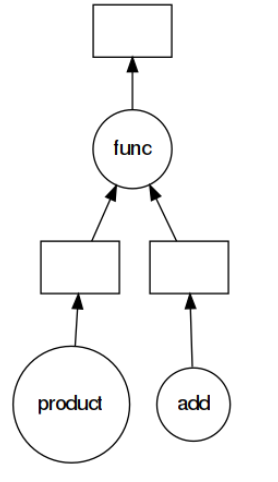
\includegraphics[scale=0.5]{figures/func.png}
\caption{\dask graph generated in Listing~\ref{listdelayed}. From the bottom to the top, we first compute the `product` and `add` functions asynchronously, and then we apply the `func` function to their results.}
\label{figfunc}
\end{figure}


\subsubsection{\dask Collections and Futures}
In addition to the \texttt{@delated} decorator, used to create task graphs, 
\dask supports parallel versions of familiar libraries such as \texttt{Numpy} and \texttt{Pandas}, respectively, \texttt{dask.array} and \texttt{dask.dataframe}, with almost similar APIs to thier sequential counterparts. 
Thus, they become usable in larger-than-memory problems. In this work, we have been particularly interested in \textit{dask.array}. 
A \textit{dask.array}\cite{rocklin_dask_2015} is a potentially larger-than-memory numpy-like array; it is constructed by aggregating blocks of \texttt{numpy} arrays called chunks. Operation on a \textit{dask.array} generates a task graph automatically, thus called a high-level collection. 

The user writes code very close to sequential one using those available APIs. A task graph can be constructed and then submitted to the scheduler by calling specific functions such as \texttt{compute}. Listing~\ref{listda} shows a \dask code, where the \texttt{dask.array} API is used alongside \texttt{@delayed}. In this example, we compute the sum of a \textit{lazy} random array. Then we apply the decorated \texttt{product} function we created in the previous example to this sum and \texttt{p}, then compute the result using the \textit{compute} method.  

\begin{lstlisting}[float=h!, label=listda, language=python, caption=Dask example using the Dask.array submodule]
import dask
import dask.array as da

# Create a random dask array of size 20*20 chunked into 5*5 blocks 
darray = da.random.random([20, 20], chunks=(5,5))

# Compute the sum of all elements in the array 
s = darray.sum()

# Visualize the created task graph 
s.visualize()

# compute the product of `s` and the computed `p` from delayed in the previous example
c = product(s, p)
result = c.compute()

# Result 
# 2456.7505213151585

\end{lstlisting}

\begin{figure}[th!]\centering

\includegraphics[scale=0.1, angle=90]{figures/func.pdf}
\caption{\dask graph generated in Listing~\ref{listda}. The circles at the bottom of the graph represent the task that will generate random data chunks. They will then be summed into partial sums, which will be aggregated to the total sum, which is then multiplied by the `p` computed in the previous example.}
\label{figda}
\end{figure}


\subsubsection{Task journey}\label{sec:taskjourney}
Task graph creation is not the only step that is done before getting to the scheduler.
Either the graph is constructed using high-level APIs or \texttt{@delayed} it goes through the following steps:
\begin{itemize}
    \item graph creation: as already presented in~\ref{sec:taskgraph}, the graph is encoded using a Python dictionary, and it may include millions of entries. This step is done on the client side, 
    \item graph optimization: \dask tries to optimize the graph and eliminate unnecessary work. This may take some time if the graph is large,
    \item graph serialization: the graph needs to be sent from the client to the scheduler and then to the workers, so it must be converted into bytes before sending it. This is done in the serialization step. 
    \item graph communication: once the graph is serialized on the client side, it is sent to the scheduler.
\end{itemize}
These steps are done after calling the \texttt{compute/persist} and may take some time if the graph is very large. 
Once the task graph is on the scheduler side, it populates its internal data structures to be able to analyze it and schedule it efficiently on the workers.

\subsubsection{Task states}\label{sec:taskstate}
In the \dask scheduler, a task can be in one of these six states: \texttt{"released", "waiting", "no-worker", "processing", "erred", "memory"}\footnote{https://distributed.dask.org/en/stable/scheduling-state.html}:

\begin{itemize}
    \item \texttt{released}: the task is known but not actively computing or in memory. Usually, a task is created in the \texttt{releard} state,

    \item \texttt{waiting}: the task is waiting on dependencies to be computed,

    \item \texttt{no-worker}: the task is ready to be computed, but no appropriate worker exists (for example, because of resource restrictions or because no worker is connected at all),

    \item \texttt{processing}: all task dependencies are available, and the task is assigned to a worker for compute (the scheduler doesn’t know whether it’s in a worker queue or actively being computed),

    \item \texttt{memory}: the task is available in the memory of one or more workers,

    \item \texttt{erred}: Task computation, or one of its dependencies, has encountered an error

    \item \texttt{forgotten}: the task is no longer needed by any client or dependent task, so it disappears from the scheduler as well. As soon as a task reaches this state, it is immediately dereferenced from the scheduler.
\end{itemize}

A task can move from one to another following stimulus coming either from a client or a worker. Figure~\ref{figdasktaskstate} shows the different states and transitions in \dask. 

\begin{figure}[h!]\centering
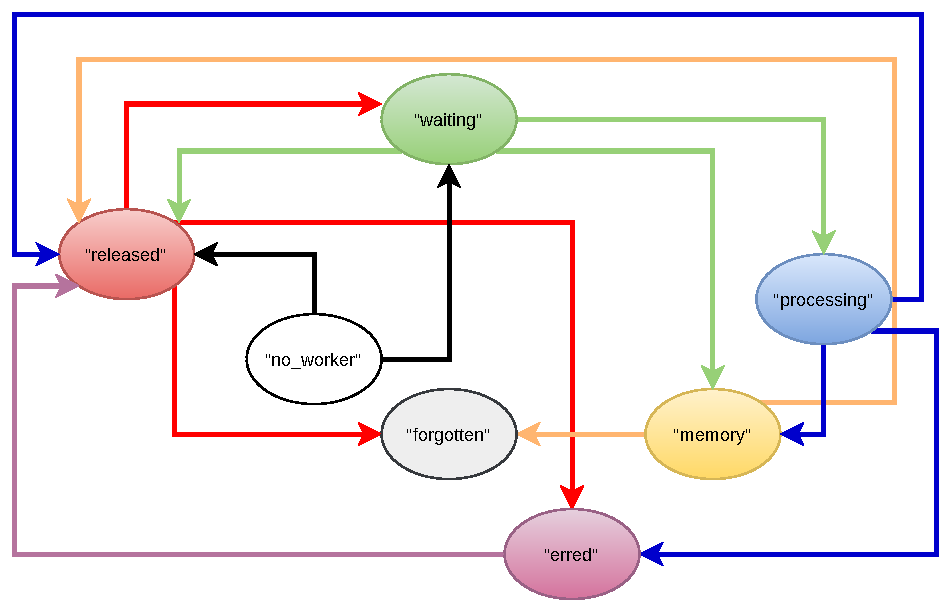
\includegraphics[scale=0.8]{figures/Dask-TaskStatesSheduler1.pdf}
\caption{\dask task states and transitions}
\label{figdasktaskstate1}
\end{figure}

And here, we will detail some transition examples. 
When a task is created, it is in the \texttt{"released"} state. It passes to the \texttt{"waiting"} state that indicates that this task is waiting for dependencies to be available in memory or it is an entry task (a task without dependencies).
If a task is an entry task, and if there are connected workers, it passes to the \texttt{"processing"} state when it is assigned to a worker.  
A task passes from the \texttt{"released"} to the \texttt{"erred"} state if a task on whom it depends erred and to the \texttt{"forgotten"} state if it is not needed anymore by an alive client or dependent task. 
When the \textit{"processing"} state is completed, it passes to the \texttt{"memory"} state and unlocks all dependent tasks. 

%The \texttt{"deisa"} has been added in the frame of this work, and it represents external pure data tasks that are arrays of data generated by a running program. More details about this state will be found in the contribution sections. 


\subsubsection{Pure Data Tasks}\label{sec:puredata}
As already mentioned, usually, the source of the data in \dask is a storage system. However, it is also possible for a client to send data to connected workers, either by passing by the scheduler or not. 
This can be done using the \texttt{scatter} method in the client API. It takes as a mandatory parameter: the data that needs to be sent and other optional parameters, such as a boolean that expresses whether or not to pass by the scheduler or a list of workers to whom the data will be sent. 
\texttt{scatter} returns a \texttt{future} to that sent data. The key of this \texttt{future} is the key of the equivalent \textit{pure data} task in the \dask scheduler. That is, the data sent via a \texttt{scatter} is also considered a task with the specificity of only containing data (without a function to be called). 


\subsection{Scheduler Internal State}\label{sec:scheduler}

The scheduler keeps track of the tasks, alive clients and connected workers in its internal data structures that consist of four main objects: the \texttt{SchedulerState}, \texttt{TaskState}, \texttt{ClientState} and \texttt{WorkerState}.
The \texttt{SchedulerState} object contains a global view of the internal state and uses the different other classes. The \texttt{TaskState} keeps the state of each task (key, state, dependencies, dependents, ...), \texttt{ClientState} and \texttt{WorkerState} keep the state of a client and a worker, respectively.
Figure~\ref{figdaskinternal} shows the four main classes in the \dask scheduler internal state and the relevant attributes to this work. 

\begin{figure}[h!]\centering
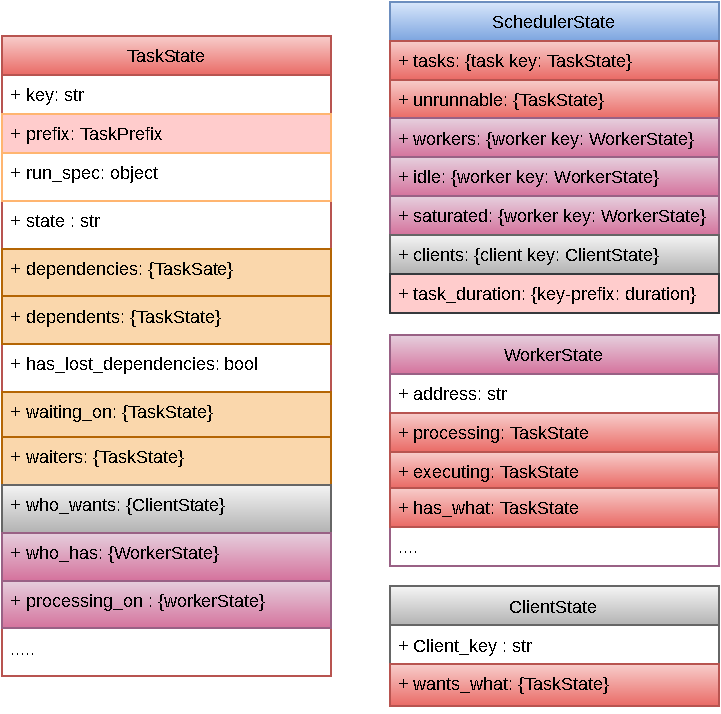
\includegraphics{figures/DaskScheduler.pdf}
\caption{\dask internal classes}
\label{figdaskinternal}
\end{figure}

We will not detail all the attributes of those classes, but understanding how they are related is important. 
For instance, in the \texttt{ClientState} class, the \texttt{wants\_what} attribute maps a client to a task from which it expects a result. The scheduler also keeps track of the tasks assigned to workers through the \texttt{WorkerState} class. The \texttt{"has\_what"} attributed. For instance, refers to task results that are in the memory of a given worker. 

The \texttt{TaskState} class is the most used in the scheduling as it keeps for each task: its dependencies (\texttt{"dependencies"}), tasks it depends on (\texttt{"dependents"}), clients that want its results (\texttt{"who\_wants"}), workers that have its result in memory is it is processed (\texttt{"who\_has"}), and the worker it is processing on if it is currently running (\texttt{"processing\_on"}). The \texttt{"waiting\_on"} is a subset of the \texttt{"dependencies"} attribute (equals at the beginning), from which we remove computed tasks. When this list is empty, and all the dependencies are completed correctly, this task passes from \texttt{"waiting"} to the \textit{"processing"}. 
The \texttt{"waiters"} keeps track of the tasks that still need this task's results. When it is empty, and no client wants it, then its results can be removed from the \dask memory.  


\subsection{Scheduling in \dask Distributed}\label{sec:scheduling}

This section does not discuss \dask scheduling policies in \dask but the \texttt{transition} algorithm, which performs state transition.
A task state transition occurs from stimuli. A stimulus is a state-changing message from a worker or a client to the scheduler. 
The scheduler handles those messages by triggering a \texttt{transition} function. Every state transition is implemented as a separate method in the scheduler. For instance, \texttt{transition\_processing\_memory} is the name of the function that performs the transition from the \textit{"processing"} to the \texttt{"memory"} state.

When a transition function is called, it mainly changes the state of the given task and constructs a dictionary of recommendations for the state transitions of other tasks, usually the depending tasks. In addition to the specific transition functions, the \texttt{transitions} method is called. As its name indicates, it triggers several transitions by iterating over the recommendations returned by the transition method. 

For example, when the scheduler receives the \texttt{"task-finished"} stimuli, the \texttt{transition\_processing\_memory} is called. It switches the task state from \texttt{"processing"} to \texttt{"memory"} and recommends all dependent tasks to switch to the \texttt{"processing"} state. These recommendations are passed to the \texttt{transitions} function that iterates over until no more recommendation is added.

A set of messages to the clients and the workers is also constructed and sent. For instance, those may contain results needed by a client or a task to be run by a worker.

\subsection{Memory Management in \dask}
\dask keeps track of all the data that are available in the workers, distributed memory. \dask has an experimental component that optimizes the memory usage of workers across, which is called Active Memory Manager\footnote{https://distributed.dask.org/en/stable/active\_memory\_manager.html}. 
We did not explore this functionality in \dask. However, we had to take into consideration the operation of the \dask's included garbage collector. 
If data is not needed anymore by any client and does not appear anymore as a dependency of any other task, then it can be deleted. To do so, \dask checks its internal data structures and updates them whenever a client or worker sends updates on it. 
For instance, if the scheduler does not receive heartbeats from a client that submitted a task graph, and those tasks are not used in other computations of other clients, the scheduler cancels them. And the garbage collector deletes the data related to those tasks from workers' memory.  

%We mention this concept because a deep understanding of how \dask manages the data is essential for further development in \dask. We will recall this concept when we need explicitly to encounter the garbage collection mechanism to keep data in \dask distributed memory. 
\subsection{Communications in \dask}
All information about where data lives in the distributed memory is kept in the scheduler's data structures. If data is needed by a worker different from the one owning it, communication between the two workers is initiated. But keep in mind that \dask scheduling policies try to schedule tasks in workers that minimize data copies. 
And worker-to-worker communications are hidden from the user's point of view, which is advantageous compared to message-passing explicit communications.

Communication between the clients is different. They are initiated by the end-user explicitly in the code. \dask provides several ways to ensure communication between clients. We focus on the coordination primitives used in our work, namely \texttt{Queues}, \texttt{Variables} and \texttt{Events}\footnote{https://docs.dask.org/en/stable/futures.html\#queues}: 

\begin{itemize}
    \item \texttt{Queue}: \dask queues follow the API for the standard Python \texttt{Queue}, but now move futures or small messages between clients. Queues send small pieces of information that are \texttt{msgpack} encodable (ints, strings, bools, lists, dictionaries, etc.). They can be used to send small metadata, and they are not adapted for sending large datasets because they are mediated by the scheduler.
    
    \item \texttt{Variable}: are like \texttt{Queues} in that they communicate futures and small data between clients. However, variables hold only a single value. The value can be \texttt{get} or \texttt{set} at any time. Variables are interesting in sharing small configurations or parameters between clients. They are also stored in the scheduler, so it is recommended to share only small data through variables.
    
    \item \texttt{Event}: hold a single flag which can be set or cleared. Clients can wait until the event flag is set. All clients can set or clear the flag, and there is no “ownership” of an event. They can be used to synchronize multiple clients.
\end{itemize}


\section{\pdi Data Interface}\label{sec:pdi}
In this section, we present the \pdi data interface, its architecture and it is used to handle our simulation data.

\subsection{Overview}\label{sec:pdioverview}

\pdi\cite{roussel:hal-01587075} data interface is a lightweight library for data handling.
It offers a declarative API to expose the data of the simulation without specifying what to do with it.
It proposes a way to call external libraries from a configuration file. 
PDI is built around three core concepts: 
\begin{itemize}
    \item data store: when data is shared from the simulation, it is made available to \pdi through the data store,
    \item event subsystem: once the data is available in the data store, the event system notifies the data handler plugin,
    \item plugins: they access the data available in the store and process it.   
\end{itemize}
The data layout, the orchestration of the exchanges, and the configuration of the different plugins are described in the specification tree; Figure~\ref {figpdiarchi} shows a structure scheme of \pdi\cite{noauthor_pdi_nodate}.  


\begin{figure}[h!]\centering
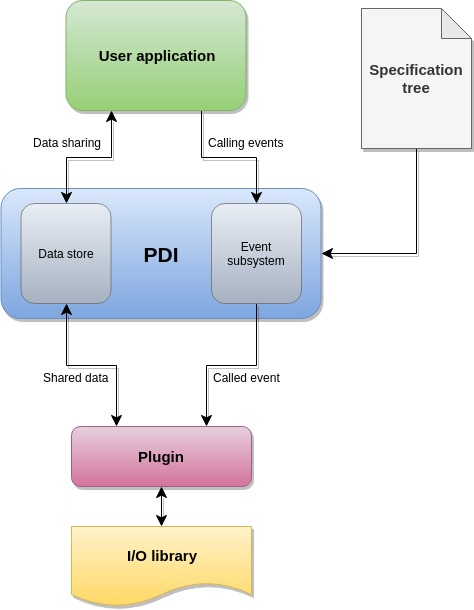
\includegraphics[scale=0.5]{figures/PDI_schema.jpg}
\caption{\pdi architecture\cite{PDI}}
\label{figpdiarchi}
\end{figure}

\subsection{\pdi API and Simulation Instrumentation}
\pdi offers a very simple API; its functions can be grouped into three categories. The initialization and finalization functions, respectively \texttt{PDI\_init} and \texttt{PDI\_finalize}, are used to set up and finalize PDI by releasing its resources. 
The second category consists of a set of functions used to annotate the code. \texttt{PDI\_share}, \texttt{PDI\_reclaim} are used to respectively share data with \pdi to be used by external plugins and reclaim it back by the simulation at the end of the plugin operation. \texttt{PDI\_expose} does both sharing and reclaiming the data from the data store. \textit{PDI\_event} triggers a PDI event and finally, \texttt{PDI\_multi\_expose} exposes several variables and triggers an event. Listing~\ref{ccode} shows an example of a c code instrumentation with \pdi, \pdi API calls are highlighted.

\begin{lstlisting}[float=h!, label=ccode, language=c, caption=\pdi instrumentation of the C simulation code]
int main( int argc, char* argv[] ) {
  MPI_Init(&argc, &argv);
  |\hlline|PDI_init(PC_parse_path("pdi_spec.yml")); |\label{ccode:PDI_init}|
  int rank; PDI_Comm_rank(MPI_COMM_WORLD, &rank);
  config_t cfg = read_config("simulation.yml");
  // share one-off configuration
  |\hlline|PDI_multi_expose("init", |\label{ccode:expose1}|
  |\hlline|    "cfg",  &cfg,  PDI_OUT, |\label{ccode:cfg}|
  |\hlline|    "rank", &rank, PDI_OUT,
  |\hlline|    NULL); |\label{ccode:expose1-end}|
  // our temperature field
  double* temp = malloc(sizeof(double) * cfg.loc[0] * cfg.loc[1]);
  initialize(temp);
  // main loop
  for (int step=0; ii<nb_steps; ++step) {
    do_compute(temp, MPI_COMM_WORLD);|\label{ccode:compute}|
    // share data at every iteration
    |\hlline|PDI_multi_expose("iter",  |\label{ccode:expose2}|
    |\hlline|    "step", &step, PDI_OUT,
    |\hlline|    "temp", temp,  PDI_OUT,
    |\hlline|    NULL); |\label{ccode:expose2-end}|
    MPI_Barrier(MPI_COMM_WORLD);|\label{ccode:barrier}|
  }
  free(temp);
  |\hlline|PDI_finalize();
  MPI_Finalize();
}
\end{lstlisting}

\subsection{\pdi Specification Tree}
As mentioned in Section~\ref{sec:pdioverview}, the specification tree describes the data layout, orchestrates interactions between the code and \pdi, and contains the plugin's configurations. It is specified in a \texttt{yaml} file and is provided to \pdi at the initialization. For instance, in Listing~\ref{ccode} line\ref{ccode:PDI_init} the configuration file name is \texttt{"pdi\_spec.yml"}. 

The specification tree contains three main sections: the \texttt{metadata}, \texttt{data} and \texttt{plugins} sections. The \texttt{metadata} section contains small variables for which \pdi keeps a copy that can, for example, include the sizes of a given array. The \texttt{data} section contains the data layout description. It defines the types of data expected in the store. Those data are not copied by \pdi; only pointers to the data are shared. Finally, the \texttt{plugins} section lists the plugins that will be loaded and their configurations. 

Listing~\ref{pdiymldata} shows an example of a \pdi \texttt{yaml} configuration file where a \texttt{types} section is added, where we can define new types such as \texttt{structures}. In this example, we find the \texttt{metadata} section in line~\ref{pdiymldata:metadata}. The \texttt{data} section starts in line~\ref{pdiymldata:data}. It provides a description of the \texttt{temp} field, (line~\ref{pdiymldata:temp}) including its type, subtype and size (respectively in lines~\ref{pdiymldata:temp.type},~\ref{pdiymldata:temp.subsize},~\ref{pdiymldata:temp.size}). 
Finally, the \texttt{plugin} section starts at line~\ref{pdiymldata:plugin}, loading one plugin: the \texttt{decl\_hdf5} plugin in line~\ref{pdiymldata:declhdf5}. The \pdi plugin system is detailed in the following.

\begin{lstlisting}[float=h!, label=pdiymldata, language=yaml, caption=Data description in \pdi YAML file]
types: #[...] including config_t description
metadata: {step: int, cfg: config_t, rank: int} |\label{pdiymldata:metadata}|
data: |\label{pdiymldata:data}|
  temp: # the main temperature field |\label{pdiymldata:temp}|
    type: array |\label{pdiymldata:temp.type}|
    subtype: double |\label{pdiymldata:temp.subsize}|
    size: [ '$cfg.loc[0]', '$cfg.loc[1]' ]  |\label{pdiymldata:temp.size}|
plugins: |\label{pdiymldata:plugin}|
  decl_hdf5: |\label{pdiymldata:declhdf5}|
  - file: data-$step-$rank.h5 
    write:
      temp:
        when: '$step>0' |\label{pdiymldata:when}|
\end{lstlisting}

\subsection{\pdi Plugins}\label{plugins}
\pdi supports loose coupling of simulation codes with external libraries. Those libraries are supported in \pdi as plugins and are configured through the specification tree. \pdi offers a list of built-in plugins ranging from IO-specific ones to more generic data handling tools. It also allows the creation of user-specific plugins if the built-in ones are not enough.     

The built-in plugins \pdi provide can be grouped into four categories: 
\begin{itemize}
    \item general purpose: include \texttt{mpi}, \texttt{trace}, \texttt{set\_value}, \texttt{pycall}, \texttt{user\_code}, \texttt{serialize},  
    \item IO: include \texttt{decl’hdf5}, \texttt{decl’NetCDF}, \texttt{SIONlib} plugins,
    \item fault tolerance: \texttt{FTI}plugin.
\end{itemize}

In Listing~\ref{pdiymldata}, one plugin have been used the \texttt{decl\_hdf5} plugin in line~\ref{pdiymldata:declhdf5}. In this example, a file named \textit{data-step-rank.h5} is written by each process in every step greater than 0. 

\pdi is extensible, and the user can add new plugins. For instance, \texttt{FlowVR}, \texttt{Melissa}, and \texttt{Sensei} plugins have been added. \texttt{FlowVR} and \texttt{Sensei} have been already presented in Section~\ref{sec:insitu:tools}, and \texttt{Melissa}\cite{terraz_melissa} is an in situ framework for sensibility analysis. 


\section{Summary}
In this chapter, we have presented the tools we chose to use in our work, namely \dask distributed and \pdi data interface.
\dask distributed has been selected for its ease of use thanks to the high-level parallel libraries it supports. We have prioritized the practicality as our goal is to bring together in situ performance and post hoc ease of use.
We have decided to keep a good separation of concerns while handling the data to maintain good habits while keeping a simple declarative interface. Thus we have opted for \pdi data handling tool to extract data from the simulation and \pdi plugins to process it. 